\documentclass[]{book}
\usepackage{lmodern}
\usepackage{amssymb,amsmath}
\usepackage{ifxetex,ifluatex}
\usepackage{fixltx2e} % provides \textsubscript
\ifnum 0\ifxetex 1\fi\ifluatex 1\fi=0 % if pdftex
  \usepackage[T1]{fontenc}
  \usepackage[utf8]{inputenc}
\else % if luatex or xelatex
  \ifxetex
    \usepackage{mathspec}
  \else
    \usepackage{fontspec}
  \fi
  \defaultfontfeatures{Ligatures=TeX,Scale=MatchLowercase}
\fi
% use upquote if available, for straight quotes in verbatim environments
\IfFileExists{upquote.sty}{\usepackage{upquote}}{}
% use microtype if available
\IfFileExists{microtype.sty}{%
\usepackage{microtype}
\UseMicrotypeSet[protrusion]{basicmath} % disable protrusion for tt fonts
}{}
\usepackage[margin=1in]{geometry}
\usepackage{hyperref}
\hypersetup{unicode=true,
            pdftitle={Podstawy programowania R},
            pdfauthor={Łukasz Wawrowski},
            pdfborder={0 0 0},
            breaklinks=true}
\urlstyle{same}  % don't use monospace font for urls
\usepackage{natbib}
\bibliographystyle{plainnat}
\usepackage{color}
\usepackage{fancyvrb}
\newcommand{\VerbBar}{|}
\newcommand{\VERB}{\Verb[commandchars=\\\{\}]}
\DefineVerbatimEnvironment{Highlighting}{Verbatim}{commandchars=\\\{\}}
% Add ',fontsize=\small' for more characters per line
\usepackage{framed}
\definecolor{shadecolor}{RGB}{248,248,248}
\newenvironment{Shaded}{\begin{snugshade}}{\end{snugshade}}
\newcommand{\KeywordTok}[1]{\textcolor[rgb]{0.13,0.29,0.53}{\textbf{#1}}}
\newcommand{\DataTypeTok}[1]{\textcolor[rgb]{0.13,0.29,0.53}{#1}}
\newcommand{\DecValTok}[1]{\textcolor[rgb]{0.00,0.00,0.81}{#1}}
\newcommand{\BaseNTok}[1]{\textcolor[rgb]{0.00,0.00,0.81}{#1}}
\newcommand{\FloatTok}[1]{\textcolor[rgb]{0.00,0.00,0.81}{#1}}
\newcommand{\ConstantTok}[1]{\textcolor[rgb]{0.00,0.00,0.00}{#1}}
\newcommand{\CharTok}[1]{\textcolor[rgb]{0.31,0.60,0.02}{#1}}
\newcommand{\SpecialCharTok}[1]{\textcolor[rgb]{0.00,0.00,0.00}{#1}}
\newcommand{\StringTok}[1]{\textcolor[rgb]{0.31,0.60,0.02}{#1}}
\newcommand{\VerbatimStringTok}[1]{\textcolor[rgb]{0.31,0.60,0.02}{#1}}
\newcommand{\SpecialStringTok}[1]{\textcolor[rgb]{0.31,0.60,0.02}{#1}}
\newcommand{\ImportTok}[1]{#1}
\newcommand{\CommentTok}[1]{\textcolor[rgb]{0.56,0.35,0.01}{\textit{#1}}}
\newcommand{\DocumentationTok}[1]{\textcolor[rgb]{0.56,0.35,0.01}{\textbf{\textit{#1}}}}
\newcommand{\AnnotationTok}[1]{\textcolor[rgb]{0.56,0.35,0.01}{\textbf{\textit{#1}}}}
\newcommand{\CommentVarTok}[1]{\textcolor[rgb]{0.56,0.35,0.01}{\textbf{\textit{#1}}}}
\newcommand{\OtherTok}[1]{\textcolor[rgb]{0.56,0.35,0.01}{#1}}
\newcommand{\FunctionTok}[1]{\textcolor[rgb]{0.00,0.00,0.00}{#1}}
\newcommand{\VariableTok}[1]{\textcolor[rgb]{0.00,0.00,0.00}{#1}}
\newcommand{\ControlFlowTok}[1]{\textcolor[rgb]{0.13,0.29,0.53}{\textbf{#1}}}
\newcommand{\OperatorTok}[1]{\textcolor[rgb]{0.81,0.36,0.00}{\textbf{#1}}}
\newcommand{\BuiltInTok}[1]{#1}
\newcommand{\ExtensionTok}[1]{#1}
\newcommand{\PreprocessorTok}[1]{\textcolor[rgb]{0.56,0.35,0.01}{\textit{#1}}}
\newcommand{\AttributeTok}[1]{\textcolor[rgb]{0.77,0.63,0.00}{#1}}
\newcommand{\RegionMarkerTok}[1]{#1}
\newcommand{\InformationTok}[1]{\textcolor[rgb]{0.56,0.35,0.01}{\textbf{\textit{#1}}}}
\newcommand{\WarningTok}[1]{\textcolor[rgb]{0.56,0.35,0.01}{\textbf{\textit{#1}}}}
\newcommand{\AlertTok}[1]{\textcolor[rgb]{0.94,0.16,0.16}{#1}}
\newcommand{\ErrorTok}[1]{\textcolor[rgb]{0.64,0.00,0.00}{\textbf{#1}}}
\newcommand{\NormalTok}[1]{#1}
\usepackage{longtable,booktabs}
\usepackage{graphicx,grffile}
\makeatletter
\def\maxwidth{\ifdim\Gin@nat@width>\linewidth\linewidth\else\Gin@nat@width\fi}
\def\maxheight{\ifdim\Gin@nat@height>\textheight\textheight\else\Gin@nat@height\fi}
\makeatother
% Scale images if necessary, so that they will not overflow the page
% margins by default, and it is still possible to overwrite the defaults
% using explicit options in \includegraphics[width, height, ...]{}
\setkeys{Gin}{width=\maxwidth,height=\maxheight,keepaspectratio}
\IfFileExists{parskip.sty}{%
\usepackage{parskip}
}{% else
\setlength{\parindent}{0pt}
\setlength{\parskip}{6pt plus 2pt minus 1pt}
}
\setlength{\emergencystretch}{3em}  % prevent overfull lines
\providecommand{\tightlist}{%
  \setlength{\itemsep}{0pt}\setlength{\parskip}{0pt}}
\setcounter{secnumdepth}{5}
% Redefines (sub)paragraphs to behave more like sections
\ifx\paragraph\undefined\else
\let\oldparagraph\paragraph
\renewcommand{\paragraph}[1]{\oldparagraph{#1}\mbox{}}
\fi
\ifx\subparagraph\undefined\else
\let\oldsubparagraph\subparagraph
\renewcommand{\subparagraph}[1]{\oldsubparagraph{#1}\mbox{}}
\fi

%%% Use protect on footnotes to avoid problems with footnotes in titles
\let\rmarkdownfootnote\footnote%
\def\footnote{\protect\rmarkdownfootnote}

%%% Change title format to be more compact
\usepackage{titling}

% Create subtitle command for use in maketitle
\newcommand{\subtitle}[1]{
  \posttitle{
    \begin{center}\large#1\end{center}
    }
}

\setlength{\droptitle}{-2em}
  \title{Podstawy programowania R}
  \pretitle{\vspace{\droptitle}\centering\huge}
  \posttitle{\par}
  \author{Łukasz Wawrowski}
  \preauthor{\centering\large\emph}
  \postauthor{\par}
  \date{}
  \predate{}\postdate{}

\usepackage{booktabs}
\usepackage{amsthm}
\makeatletter
\def\thm@space@setup{%
  \thm@preskip=8pt plus 2pt minus 4pt
  \thm@postskip=\thm@preskip
}
\makeatother

\begin{document}
\maketitle

{
\setcounter{tocdepth}{1}
\tableofcontents
}
\chapter*{Wprowadzenie}\label{wprowadzenie}
\addcontentsline{toc}{chapter}{Wprowadzenie}

Literatura podstawowa:

\begin{itemize}
\tightlist
\item
  Przemysław Biecek -
  \href{http://pbiecek.github.io/Przewodnik/}{\emph{Przewodnik po
  pakiecie R}}
\item
  Marek Gągolewski -
  \href{http://www.gagolewski.com/publications/programowanier/}{\emph{Programowanie
  w języku R. Analiza danych, obliczenia, symulacje.}}
\item
  Garret Grolemund, Hadley Wickham -
  \href{http://r4ds.had.co.nz/}{\emph{R for Data Science}}
  (\href{link}{polska wersja})
\end{itemize}

Literatura dodatkowa:

\begin{itemize}
\tightlist
\item
  \href{https://github.com/mi2-warsaw/SER/blob/master/histoRia/README.md}{inne
  pozycje po polsku}
\item
  \href{https://bookdown.org/}{inne pozycje po angielsku}
\end{itemize}

Internet:

\begin{itemize}
\tightlist
\item
  \href{https://www.r-bloggers.com/}{R-bloggers}
\item
  \href{https://rweekly.org/}{rweekly}
\end{itemize}

\chapter{Wprowadzenie do R}\label{wprowadzenie-do-r}

GNU R to interpretowany język programowania oraz środowisko do obliczeń
statystycznych i wizualizacji wyników {[}Wikipedia 2017{]}.

Robert A. Muenchen - \href{http://r4stats.com/articles/popularity/}{The
Popularity of Data Science Software}

\begin{figure}
\centering
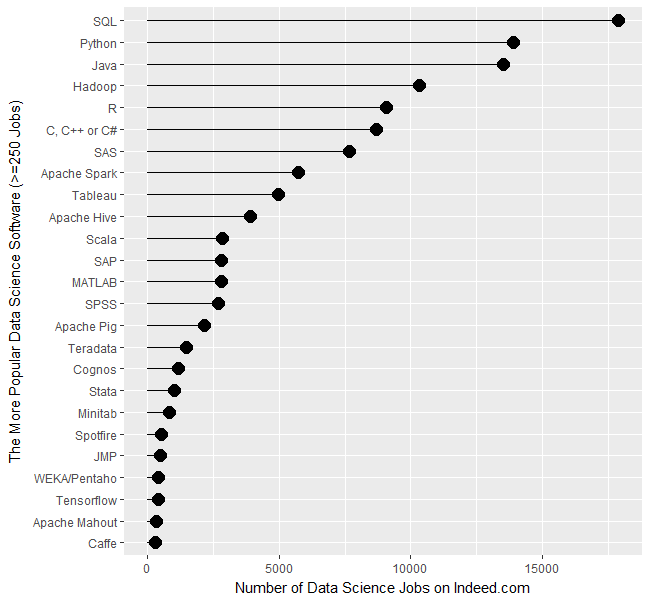
\includegraphics{img/pop_r1.png}
\caption{}
\end{figure}

\section{R}\label{r}

Bazowa wersja R jest do pobrania ze strony
\href{https://cloud.r-project.org/}{r-project.org}.

\begin{figure}
\centering
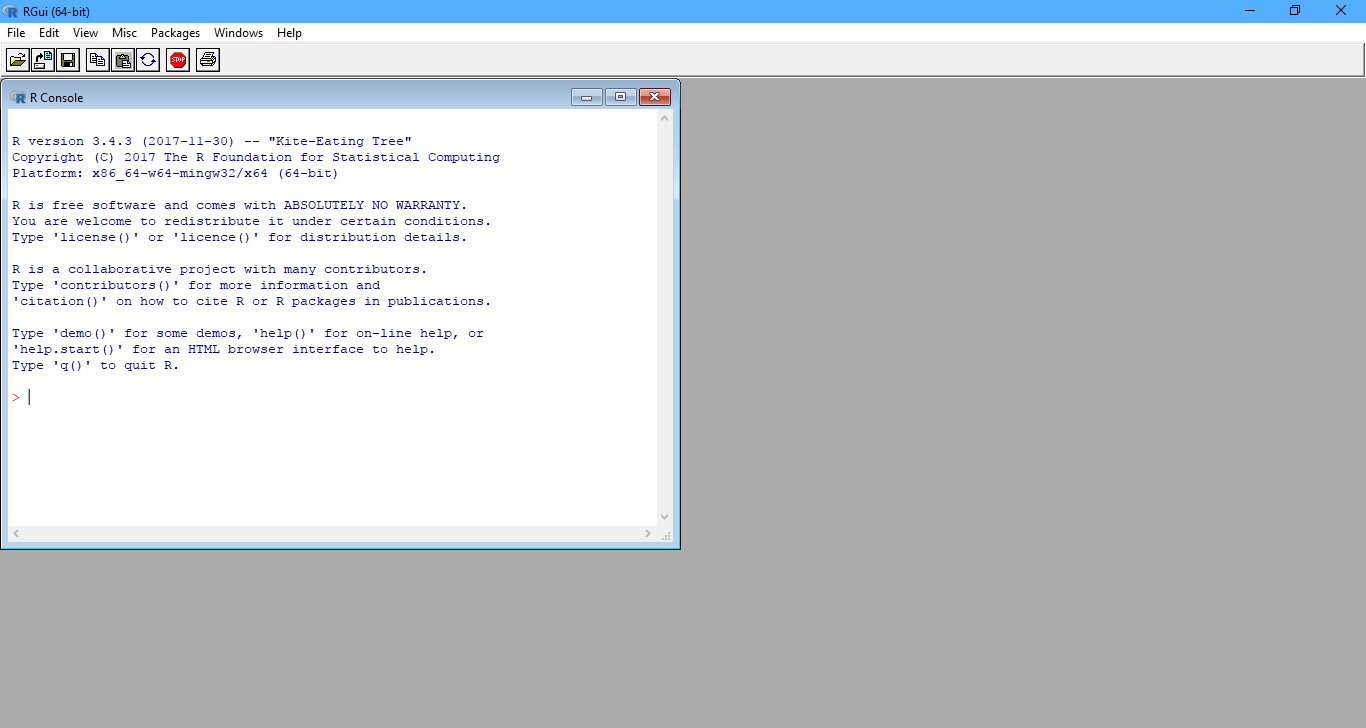
\includegraphics{img/r.png}
\caption{}
\end{figure}

\section{RStudio}\label{rstudio}

RStudio to zintegrowane środowisko programistyczne (IDE) dla języka R
dostępne za darmo na stronie
\href{https://www.rstudio.com/products/rstudio/download/}{RStudio}.

\begin{figure}
\centering
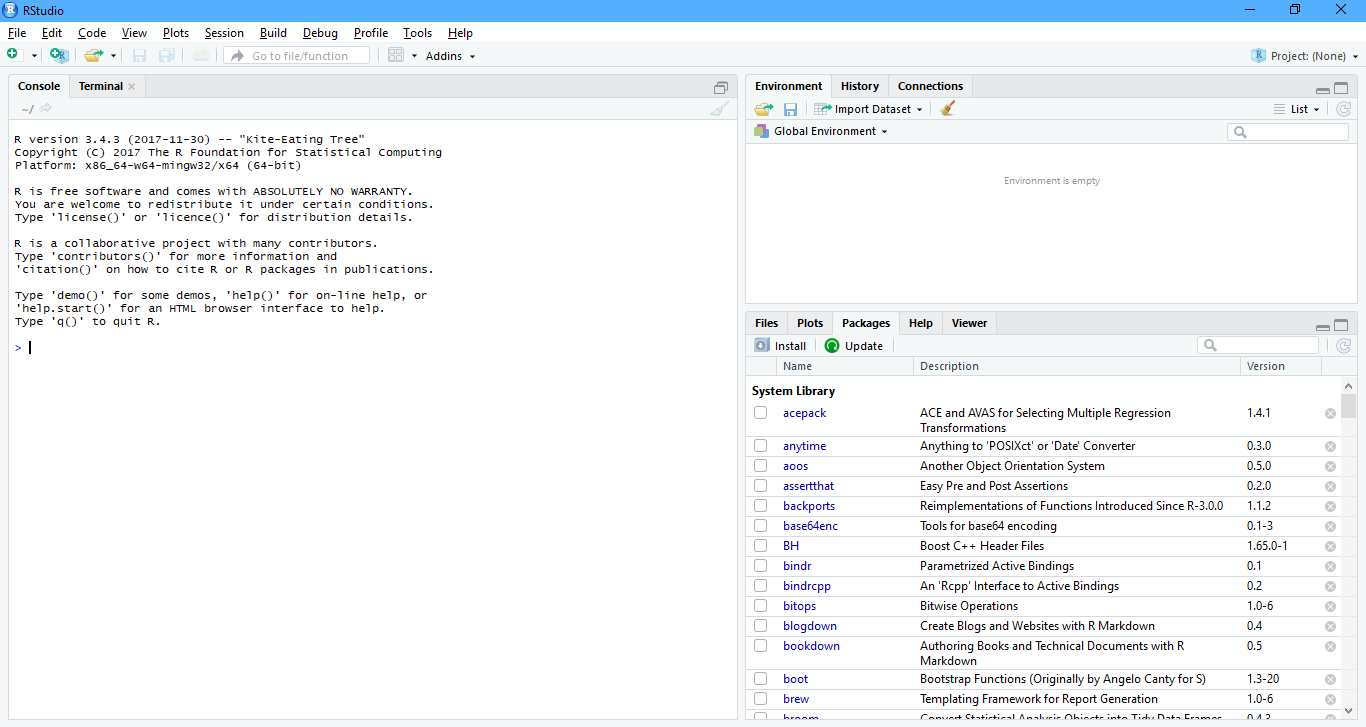
\includegraphics{img/rstudio.png}
\caption{}
\end{figure}

Z R można także korzystać w
\href{https://www.visualstudio.com/pl/vs/rtvs/}{Microsoft Visual
Studio}.

\section{Ważne informacje}\label{wazne-informacje}

\textbf{R jest wrażliwy na wielkość liter.}

\textbf{Separatorem części dziesiętnej liczby jest kropka.}

\textbf{W codziennej pracy RStudio jest wygodniejsze, jednak długotrwałe
obliczenia lepiej uruchamiać w trybie wsadowym w zwykłym R.}

\begin{itemize}
\tightlist
\item
  \textbf{Katalog roboczy}
\end{itemize}

Ważnym pojęciem w R jest katalog roboczy (ang. working directory), który
określa gdzie zostaną zapisane pliki, wykresy, zbiory, itp. jeśli nie
podamy dokładnej ścieżki do pliku. Katalog roboczy przypisuje się z
wykorzystaniem funkcji \texttt{setwd("ścieżka\ do\ katalogu")}, a jego
wartość można sprawdzić funkcją \texttt{getwd()}. W RStudio przypisanie
katalogu roboczego odbywa się w momencie utworzenia projektu.

\begin{itemize}
\tightlist
\item
  \textbf{Projekt}
\end{itemize}

Katalog na dysku, w którym znajdują się wszystkie pliki projektu wraz z
plikiem o rozszerzeniu .Rproj skojarzonym z RStudio.

\begin{itemize}
\tightlist
\item
  \textbf{Korzystanie z pomocy}
\end{itemize}

Dostęp do pomocy odnośnie wybranej funkcji można uzyskać na dwa sposoby.
Pierwszym z nich jest poprzedzenie nazwy funkcji w konsoli znakiem
zapytania np. \texttt{?getwd} lub wywołanie funkcji help na nazwie
funkcji \texttt{help("getwd")}. Drugim sposobem jest umieszczenie
kursora w dowolnym miejscu nazwy funkcji i wciśnięcie klawisza F1.

Internet - przede wszystkim
\href{https://stackoverflow.com/questions/tagged/r}{stackoverflow}.

\begin{itemize}
\tightlist
\item
  \textbf{Komentarze}
\end{itemize}

\begin{quote}
Real programmers don't comment their code. If it was hard to write it
should be hard to understand.
\end{quote}

Dobrze napisany kod jest czytelny bez komentarzy. W R komentarze
rozpoczynają się od symbolu \#. Skrót klawiaturowy w RStudio to CTRL +
SHIFT + C (do wstawiania i usuwania komentarzy).

\begin{itemize}
\tightlist
\item
  \textbf{Podpowiadanie składni}
\end{itemize}

RStudio ma zaimplementowaną funkcję podpowiadania składni. Listę
możliwych funkcji i obiektów wywołuję się klawiszem TAB lub CTRL +
SPACJA po wpisaniu co najmniej jednej litery. Kolejne naciśnięcie TAB
lub ENTER powoduje uzupełnienie kodu o wybraną funkcję lub obiekt.

\begin{itemize}
\tightlist
\item
  \textbf{Wykonywanie programów}
\end{itemize}

Programy w R możemy tworzyć jako skrypty w pliku tekstowym o
rozszerzeniu .R lub wywoływać polecenia bezpośrednio w konsoli. Kod
programu napisanego w skrypcie przekazywany jest do konsoli. Gotowość do
pracy R sygnalizuje w konsoli znakiem zachęty \texttt{\textgreater{}}.
Jeśli podczas wykonywania programu w konsoli pojawi się znak \texttt{+}
to oznacza oczekiwanie na kompletny kod - brak domkniętego nawiasu,
cudzysłowia, itp.:

\begin{verbatim}
> getwd(
+ 
\end{verbatim}

W powyższym przykładzie brakuje prawego nawiasu. Dodanie brakującego
kodu spowoduje wykonanie przekazanego polecenia. Z kolei wciśnięcie
klawisza ESC spowoduje przerwanie wykonywanie programu i powrót do znaku
zachęty. Zawartość konsoli można wyczyścić stosując kombinację klawiszy
CTRL + L.

\begin{itemize}
\tightlist
\item
  \textbf{Pliki }
\end{itemize}

Jeśli w pamięci znajdują się jakieś obiekty (zakładka Environment) to
RStudio przy zamykaniu programu zapyta o zapisanie tych obiektów do
pliku .RData. Jeżeli zdecydujemy się na tą propozycję to po ponownym
uruchomieniu projektu obiekty znajdujące się w pliku .RData zostaną
automatycznie wczytane do pamięci.

Można także samodzielnie tworzyć pliki o rozszerzeniu .RData z
wykorzystaniem funkcji \texttt{save()}:

\begin{verbatim}
save(obiekt1, obiekt2, obiekt3, file = "nazwa_pliku.RData")
\end{verbatim}

Wczytanie obiektów z takiego pliku do pamięci odbywa się z zastosowaniem
funkcji \texttt{load()}:

\begin{verbatim}
load("nazwa_pliku.RData")
\end{verbatim}

\section{Pakiety}\label{pakiety}

Podstawowe możliwości R są dosyć ograniczone. Rozszerzają je pakiety,
których obecnie jest ponad 12 tysięcy. Można je przeglądać według
kategorii w \href{https://cran.r-project.org/web/views/}{CRAN Task
Views} lub w wygodnej wyszukiwarce
\href{https://www.r-pkg.org/}{METACRAN} i
\href{https://rdrr.io/}{rdrr.io}.

\section{R jako kalkulator}\label{r-jako-kalkulator}

Działania matematycznie w R:

\begin{longtable}[]{@{}cc@{}}
\toprule
Operator & Operacja\tabularnewline
\midrule
\endhead
+ & dodawanie\tabularnewline
- & odejmowanie\tabularnewline
* & mnożenie\tabularnewline
/ & dzielenie\tabularnewline
\^{} lub ** & potęgowanie\tabularnewline
sqrt() & pierwiastkowanie\tabularnewline
\bottomrule
\end{longtable}

W R istnieje także stała wbudowana \texttt{pi} przechowująca wartość
liczby pi.

Funkcja \texttt{factorial(x)} zwraca silnię (znak wykrzyknika !) z
podanej wartości x, a \texttt{sign(x)} sprawdza znak wyrażenia i zwraca
odpowiednio wartość -1 jeśli wyrażenie jest ujemne, 0 jeśli jest równe 0
i 1 dla wyrażeń dodatnich.

Funkcja \texttt{exp(x)} zwraca wartość wyrażenia \(e^x\), natomiast
funkcja \texttt{log(x)} zwraca logarytm z podanej liczby. Domyślnie jest
to logarytm naturalny, ale można zmienić podstawę podając wartość
argumentu \texttt{base}.

Funkcja \texttt{abs(x)} zwraca wartość bezwzględną (absolutną)
wyrażenia.

\textbf{Ćwiczenie}

Oblicz wartość wyrażenia: \(2\cdot \sqrt{\pi} + log_28\).

Rozwiązanie:

\begin{Shaded}
\begin{Highlighting}[]
\DecValTok{2}\OperatorTok{*}\KeywordTok{sqrt}\NormalTok{(pi)}\OperatorTok{+}\KeywordTok{log}\NormalTok{(}\DecValTok{8}\NormalTok{,}\DecValTok{2}\NormalTok{)}
\end{Highlighting}
\end{Shaded}

\begin{verbatim}
## [1] 6.544908
\end{verbatim}

\textbf{Zadania}

Oblicz wartość wyrażeń:

\begin{enumerate}
\def\labelenumi{\arabic{enumi}.}
\tightlist
\item
  \(\frac{2^3\cdot6^2}{(\frac{1}{2})^2\cdot(\frac{4}{5})^3}\)
\item
  \(\sqrt[3]{\frac{6-3.5}{2^{11}}}\)
\item
  \(\pi+\sqrt{e^4}\)
\item
  \(5! - log_{10}100\)
\item
  \(|1-e|\)
\end{enumerate}

\chapter{Struktury danych}\label{struktury-danych}

W R praktycznie wszystko jest obiektem. Może to być zbiór danych, ale
także wykres czy mapa. Zasadnicza różnica to klasa tych obiektów i
operacje jakie mogą być na nich wykonywane.

Funkcje w R wymagają jako argumentów określonych typów obiektów - stąd
tak ważna jak znajomość istniejących struktur.

Każdy obiekt w R możemy przypisać do tzw. obiektu nazwanego. Wówczas
jest przechowywany w pamięci i można się do niego odwołać. Przypisanie
odbywa się za pomocą operatora \texttt{\textless{}-}.

\begin{verbatim}
nazwa <- obiekt
obiekt -> nazwa
\end{verbatim}

Można także przypisywać obiekty z wykorzystaniem znaku równości
\texttt{=}, ale nie jest to zalecane ponieważ symbol ten jest używany w
innych miejscach np. do deklarowania wartości argumentów w funkcji.

W R dostępna jest funkcja \texttt{assign}, która także umożliwia
przypisanie nazwy do obiektu:

\begin{verbatim}
assign("nazwa", obiekt)
\end{verbatim}

\section{Wektor}\label{wektor}

Wektor jest najprostszym typem danych w R. Najczęściej korzysta się z
trzech typów wektorów:

\begin{itemize}
\tightlist
\item
  logicznych
\item
  liczbowych
\item
  tekstowych
\end{itemize}

Wektor tworzy się z wykorzystaniem funkcji \texttt{c()}.

\subsection{Wektor wartości
logicznych}\label{wektor-wartosci-logicznych}

Przyjmuje wartości \emph{prawda} lub \emph{fałsz}:

\begin{Shaded}
\begin{Highlighting}[]
\KeywordTok{c}\NormalTok{(}\OtherTok{TRUE}\NormalTok{, }\OtherTok{FALSE}\NormalTok{, }\OtherTok{FALSE}\NormalTok{)}
\end{Highlighting}
\end{Shaded}

\begin{verbatim}
## [1]  TRUE FALSE FALSE
\end{verbatim}

lub w skróconej wersji:

\begin{Shaded}
\begin{Highlighting}[]
\KeywordTok{c}\NormalTok{(T, F, F)}
\end{Highlighting}
\end{Shaded}

\begin{verbatim}
## [1]  TRUE FALSE FALSE
\end{verbatim}

Do sprawdzenia długości wektora używa się funkcji \texttt{length}:

\begin{Shaded}
\begin{Highlighting}[]
\KeywordTok{length}\NormalTok{(}\KeywordTok{c}\NormalTok{(T, F, F))}
\end{Highlighting}
\end{Shaded}

\begin{verbatim}
## [1] 3
\end{verbatim}

lub korzystając z obiektu nazwanego:

\begin{Shaded}
\begin{Highlighting}[]
\NormalTok{wart_log <-}\StringTok{ }\KeywordTok{c}\NormalTok{(T,F,F)}
\KeywordTok{length}\NormalTok{(wart_log)}
\end{Highlighting}
\end{Shaded}

\begin{verbatim}
## [1] 3
\end{verbatim}

Wektory można także utworzyć poprzez replikację określonej wartości lub
wektora z wykorzystaniem funkcji \texttt{rep}. Funkcja ta przyjmuje co
najmniej dwa argumenty: obowiązkowo \texttt{x} - wektor wejściowy oraz
jeden z następujących: \texttt{times} - liczba powtórzeń elementów
wektora \texttt{x}, \texttt{each} - liczba powtórzeń elementów wektora
\texttt{x} (wyjaśnienie różnicy poniżej) lub \texttt{length.out} -
oczekiwana długość wektora wynikowego.

Trzy równoważne zapisy:

\begin{Shaded}
\begin{Highlighting}[]
\KeywordTok{rep}\NormalTok{(}\DataTypeTok{x =} \KeywordTok{c}\NormalTok{(T,F), }\DataTypeTok{times =} \DecValTok{3}\NormalTok{)}
\end{Highlighting}
\end{Shaded}

\begin{verbatim}
## [1]  TRUE FALSE  TRUE FALSE  TRUE FALSE
\end{verbatim}

\begin{Shaded}
\begin{Highlighting}[]
\KeywordTok{rep}\NormalTok{(}\KeywordTok{c}\NormalTok{(T,F), }\DataTypeTok{times =} \DecValTok{3}\NormalTok{)}
\end{Highlighting}
\end{Shaded}

\begin{verbatim}
## [1]  TRUE FALSE  TRUE FALSE  TRUE FALSE
\end{verbatim}

\begin{Shaded}
\begin{Highlighting}[]
\KeywordTok{rep}\NormalTok{(}\KeywordTok{c}\NormalTok{(T,F), }\DecValTok{3}\NormalTok{)}
\end{Highlighting}
\end{Shaded}

\begin{verbatim}
## [1]  TRUE FALSE  TRUE FALSE  TRUE FALSE
\end{verbatim}

A tak to wygląda z argumentem \texttt{each}:

\begin{Shaded}
\begin{Highlighting}[]
\KeywordTok{rep}\NormalTok{(}\KeywordTok{c}\NormalTok{(T,F), }\DataTypeTok{each =} \DecValTok{3}\NormalTok{)}
\end{Highlighting}
\end{Shaded}

\begin{verbatim}
## [1]  TRUE  TRUE  TRUE FALSE FALSE FALSE
\end{verbatim}

Wykorzystanie argumentu \texttt{length.out}:

\begin{Shaded}
\begin{Highlighting}[]
\KeywordTok{rep}\NormalTok{(}\KeywordTok{c}\NormalTok{(T,F), }\DataTypeTok{length.out =} \DecValTok{5}\NormalTok{)}
\end{Highlighting}
\end{Shaded}

\begin{verbatim}
## [1]  TRUE FALSE  TRUE FALSE  TRUE
\end{verbatim}

\subsection{Wektor wartości
liczbowych}\label{wektor-wartosci-liczbowych}

W wektorze możemy przechowywać także liczby:

\begin{Shaded}
\begin{Highlighting}[]
\KeywordTok{c}\NormalTok{(}\DecValTok{1}\NormalTok{, }\DecValTok{3}\NormalTok{, }\OperatorTok{-}\DecValTok{5}\NormalTok{, }\FloatTok{2.5}\NormalTok{, .}\DecValTok{6}\NormalTok{) }\CommentTok{# nie trzeba pisać zera przed ułamkiem}
\end{Highlighting}
\end{Shaded}

\begin{verbatim}
## [1]  1.0  3.0 -5.0  2.5  0.6
\end{verbatim}

Połączenie dwóch wektorów to także wektor:

\begin{Shaded}
\begin{Highlighting}[]
\KeywordTok{c}\NormalTok{(}\KeywordTok{c}\NormalTok{(}\DecValTok{1}\NormalTok{,}\DecValTok{2}\NormalTok{,}\DecValTok{3}\NormalTok{), }\KeywordTok{c}\NormalTok{(}\FloatTok{3.5}\NormalTok{,}\DecValTok{4}\NormalTok{,}\FloatTok{4.5}\NormalTok{))}
\end{Highlighting}
\end{Shaded}

\begin{verbatim}
## [1] 1.0 2.0 3.0 3.5 4.0 4.5
\end{verbatim}

Pojedyncza liczba też jest jednoelementowym wektorem:

\begin{Shaded}
\begin{Highlighting}[]
\KeywordTok{length}\NormalTok{(}\DecValTok{2}\NormalTok{)}
\end{Highlighting}
\end{Shaded}

\begin{verbatim}
## [1] 1
\end{verbatim}

Proste ciągi o różnicy równej 1 można generować wykorzystując dwukropek:

\begin{Shaded}
\begin{Highlighting}[]
\DecValTok{1}\OperatorTok{:}\DecValTok{10}
\end{Highlighting}
\end{Shaded}

\begin{verbatim}
##  [1]  1  2  3  4  5  6  7  8  9 10
\end{verbatim}

lub

\begin{Shaded}
\begin{Highlighting}[]
\KeywordTok{c}\NormalTok{(}\OperatorTok{-}\DecValTok{5}\OperatorTok{:-}\DecValTok{1}\NormalTok{,}\DecValTok{1}\OperatorTok{:}\DecValTok{5}\NormalTok{)}
\end{Highlighting}
\end{Shaded}

\begin{verbatim}
##  [1] -5 -4 -3 -2 -1  1  2  3  4  5
\end{verbatim}

Do generowania ciągów liczbowych o różnych różnicach wykorzystuje się
funkcję \texttt{seq}, która przyjmuje następujące argumenty. Wartość
początkową \texttt{from}, wartość końcową \texttt{to} oraz jeden z
następujących: \texttt{by} - krok lub \texttt{length.out} - oczekiwana
długość wektora.

To samo co \texttt{1:10}

\begin{Shaded}
\begin{Highlighting}[]
\KeywordTok{seq}\NormalTok{(}\DecValTok{1}\NormalTok{, }\DecValTok{10}\NormalTok{, }\DecValTok{1}\NormalTok{)}
\end{Highlighting}
\end{Shaded}

\begin{verbatim}
##  [1]  1  2  3  4  5  6  7  8  9 10
\end{verbatim}

Wartości niecałkowite:

\begin{Shaded}
\begin{Highlighting}[]
\KeywordTok{seq}\NormalTok{(}\DecValTok{1}\NormalTok{, }\DecValTok{2}\NormalTok{, }\FloatTok{0.2}\NormalTok{)}
\end{Highlighting}
\end{Shaded}

\begin{verbatim}
## [1] 1.0 1.2 1.4 1.6 1.8 2.0
\end{verbatim}

Wektor wartości malejących:

\begin{Shaded}
\begin{Highlighting}[]
\KeywordTok{seq}\NormalTok{(}\DecValTok{10}\NormalTok{, }\DecValTok{1}\NormalTok{, }\DataTypeTok{by=}\DecValTok{1}\NormalTok{) }\CommentTok{# błędny zapis}
\end{Highlighting}
\end{Shaded}

\begin{verbatim}
## Error in seq.default(10, 1, by = 1): wrong sign in 'by' argument
\end{verbatim}

\begin{Shaded}
\begin{Highlighting}[]
\KeywordTok{seq}\NormalTok{(}\DecValTok{10}\NormalTok{, }\DecValTok{1}\NormalTok{, }\DataTypeTok{by=}\OperatorTok{-}\DecValTok{1}\NormalTok{) }\CommentTok{# poprawny zapis}
\end{Highlighting}
\end{Shaded}

\begin{verbatim}
##  [1] 10  9  8  7  6  5  4  3  2  1
\end{verbatim}

Tworzenie wektora w oparciu o argument \texttt{length.out} - funkcja
sama dobiera krok:

\begin{Shaded}
\begin{Highlighting}[]
\KeywordTok{seq}\NormalTok{(}\DecValTok{1}\NormalTok{, }\DecValTok{7}\NormalTok{, }\DataTypeTok{length.out =} \DecValTok{13}\NormalTok{)}
\end{Highlighting}
\end{Shaded}

\begin{verbatim}
##  [1] 1.0 1.5 2.0 2.5 3.0 3.5 4.0 4.5 5.0 5.5 6.0 6.5 7.0
\end{verbatim}

Do generowania liczb pseudolosowych służy funkcja \texttt{runif(n)},
która do poprawnego wywołania wymaga tylko jednego argumentu - długości
wektora wynikowego. Domyślnie losowane są liczby z przedziału \([0;1]\)
(tak jak w funkcji \texttt{los()} w Excelu), można to jednak zmienić
podając odpowiednie wartości argumentów \texttt{min} i \texttt{max}.

\begin{Shaded}
\begin{Highlighting}[]
\KeywordTok{runif}\NormalTok{(}\DecValTok{6}\NormalTok{)}
\end{Highlighting}
\end{Shaded}

\begin{verbatim}
## [1] 0.1682750 0.1150516 0.6388988 0.5143479 0.3864002 0.3169787
\end{verbatim}

Obserwacje można także generować z innych rozkładów:

\begin{itemize}
\tightlist
\item
  \texttt{rnorm} - rozkład normalny,
\item
  \texttt{rchisq} - rozkład \(\chi^2\),
\item
  \texttt{rt} - rozkład t-studenta,
\item
  itp.
\end{itemize}

Wykaz wszystkich dostępnych w R rozkładów uzyskamy wywołując polecenie
\texttt{help("Distributions")}.

Za każdym uruchomieniem jednej z wymienionych wyżej funkcji losujących
wartości z danego rozkładu otrzymamy inne wartości:

\begin{Shaded}
\begin{Highlighting}[]
\KeywordTok{runif}\NormalTok{(}\DecValTok{5}\NormalTok{)}
\end{Highlighting}
\end{Shaded}

\begin{verbatim}
## [1] 0.65230048 0.74790898 0.81707627 0.06448738 0.68133472
\end{verbatim}

\begin{Shaded}
\begin{Highlighting}[]
\KeywordTok{runif}\NormalTok{(}\DecValTok{5}\NormalTok{)}
\end{Highlighting}
\end{Shaded}

\begin{verbatim}
## [1] 0.58448601 0.02847448 0.28051954 0.36799795 0.84602875
\end{verbatim}

Powtarzalność wyników możemy uzyskać ustalając ziarno generatora:

\begin{Shaded}
\begin{Highlighting}[]
\KeywordTok{set.seed}\NormalTok{(}\DecValTok{123}\NormalTok{)}
\KeywordTok{runif}\NormalTok{(}\DecValTok{5}\NormalTok{)}
\end{Highlighting}
\end{Shaded}

\begin{verbatim}
## [1] 0.2875775 0.7883051 0.4089769 0.8830174 0.9404673
\end{verbatim}

\begin{Shaded}
\begin{Highlighting}[]
\KeywordTok{set.seed}\NormalTok{(}\DecValTok{123}\NormalTok{)}
\KeywordTok{runif}\NormalTok{(}\DecValTok{5}\NormalTok{)}
\end{Highlighting}
\end{Shaded}

\begin{verbatim}
## [1] 0.2875775 0.7883051 0.4089769 0.8830174 0.9404673
\end{verbatim}

\subsection{Wektor wartości
tekstowych}\label{wektor-wartosci-tekstowych}

W wektorze może być przechowywany tekst - wówczas poszczególne elementy
zapisujemy w cudzysłowie lub apostrofach:

\begin{Shaded}
\begin{Highlighting}[]
\KeywordTok{c}\NormalTok{(}\StringTok{"ala"}\NormalTok{, }\StringTok{"ma"}\NormalTok{, }\StringTok{"kota"}\NormalTok{)}
\end{Highlighting}
\end{Shaded}

\begin{verbatim}
## [1] "ala"  "ma"   "kota"
\end{verbatim}

\begin{Shaded}
\begin{Highlighting}[]
\KeywordTok{c}\NormalTok{(}\StringTok{'ala'}\NormalTok{, }\StringTok{'ma'}\NormalTok{, }\StringTok{'kota'}\NormalTok{)}
\end{Highlighting}
\end{Shaded}

\begin{verbatim}
## [1] "ala"  "ma"   "kota"
\end{verbatim}

W RStudio wygodniej używać cudzysłowu, ponieważ program automatycznie go
zamyka.

Istnieje także stała zawierająca litery alfabetu:

\begin{Shaded}
\begin{Highlighting}[]
\NormalTok{letters}
\end{Highlighting}
\end{Shaded}

\begin{verbatim}
##  [1] "a" "b" "c" "d" "e" "f" "g" "h" "i" "j" "k" "l" "m" "n" "o" "p" "q"
## [18] "r" "s" "t" "u" "v" "w" "x" "y" "z"
\end{verbatim}

\begin{Shaded}
\begin{Highlighting}[]
\NormalTok{LETTERS}
\end{Highlighting}
\end{Shaded}

\begin{verbatim}
##  [1] "A" "B" "C" "D" "E" "F" "G" "H" "I" "J" "K" "L" "M" "N" "O" "P" "Q"
## [18] "R" "S" "T" "U" "V" "W" "X" "Y" "Z"
\end{verbatim}

\subsection{Przeciążanie wektora}\label{przeciazanie-wektora}

Jeśli w wektorze pomieszamy kilka typów zmiennych to R przekształci
poszczególne wartości, tak aby stracić jak najmniej informacji:

\begin{Shaded}
\begin{Highlighting}[]
\KeywordTok{c}\NormalTok{(}\OtherTok{TRUE}\NormalTok{, }\DecValTok{2}\NormalTok{, }\DecValTok{5}\NormalTok{)}
\end{Highlighting}
\end{Shaded}

\begin{verbatim}
## [1] 1 2 5
\end{verbatim}

\begin{Shaded}
\begin{Highlighting}[]
\KeywordTok{c}\NormalTok{(}\DecValTok{3}\NormalTok{, }\StringTok{"cztery"}\NormalTok{, }\DecValTok{5}\NormalTok{)}
\end{Highlighting}
\end{Shaded}

\begin{verbatim}
## [1] "3"      "cztery" "5"
\end{verbatim}

W pierwszym przypadku wartość \texttt{TRUE} została przekształcona na
odpowiednik liczbowy - 1. Z kolei w drugim przykładzie podane liczby
zostały przekonwertowane na tekst.

\subsection{Operacje na wektorach}\label{operacje-na-wektorach}

Na wektorach logicznych i liczbowych można wykonywać operacje
arytmetyczne np. mnożenie:

\begin{Shaded}
\begin{Highlighting}[]
\DecValTok{1}\OperatorTok{:}\DecValTok{10}\OperatorTok{*}\DecValTok{2}
\end{Highlighting}
\end{Shaded}

\begin{verbatim}
##  [1]  2  4  6  8 10 12 14 16 18 20
\end{verbatim}

Wektor liczbowy plus wektor liczbowy:

\begin{Shaded}
\begin{Highlighting}[]
\DecValTok{1}\OperatorTok{:}\DecValTok{10} \OperatorTok{+}\StringTok{ }\KeywordTok{c}\NormalTok{(}\DecValTok{1}\NormalTok{,}\DecValTok{2}\NormalTok{)}
\end{Highlighting}
\end{Shaded}

\begin{verbatim}
##  [1]  2  4  4  6  6  8  8 10 10 12
\end{verbatim}

Wektor liczbowy razy wektor liczbowy:

\begin{Shaded}
\begin{Highlighting}[]
\DecValTok{1}\OperatorTok{:}\DecValTok{10} \OperatorTok{*}\StringTok{ }\KeywordTok{c}\NormalTok{(}\DecValTok{1}\NormalTok{,}\DecValTok{2}\NormalTok{)}
\end{Highlighting}
\end{Shaded}

\begin{verbatim}
##  [1]  1  4  3  8  5 12  7 16  9 20
\end{verbatim}

Wektor liczbowy razy wektor logiczny:

\begin{Shaded}
\begin{Highlighting}[]
\DecValTok{1}\OperatorTok{:}\DecValTok{10} \OperatorTok{*}\StringTok{ }\KeywordTok{c}\NormalTok{(T, F)}
\end{Highlighting}
\end{Shaded}

\begin{verbatim}
##  [1] 1 0 3 0 5 0 7 0 9 0
\end{verbatim}

Długości obu wektorów muszą być odpowiednie:

\begin{Shaded}
\begin{Highlighting}[]
\DecValTok{1}\OperatorTok{:}\DecValTok{10} \OperatorTok{*}\StringTok{ }\KeywordTok{c}\NormalTok{(T,F,T)}
\end{Highlighting}
\end{Shaded}

\begin{verbatim}
## Warning in 1:10 * c(T, F, T): longer object length is not a multiple of
## shorter object length
\end{verbatim}

\begin{verbatim}
##  [1]  1  0  3  4  0  6  7  0  9 10
\end{verbatim}

Dłuższy z wektorów musi być wielokrotnością krótszego.

Siłą rzeczy działania arytmetyczne na wektorach tekstowych nie są
możliwe:

\begin{Shaded}
\begin{Highlighting}[]
\KeywordTok{c}\NormalTok{(}\StringTok{"jeden"}\NormalTok{, }\StringTok{"dwa"}\NormalTok{, }\StringTok{"trzy"}\NormalTok{, }\StringTok{"cztery"}\NormalTok{) }\OperatorTok{*}\StringTok{ }\KeywordTok{c}\NormalTok{(T,F)}
\end{Highlighting}
\end{Shaded}

\begin{verbatim}
## Error in c("jeden", "dwa", "trzy", "cztery") * c(T, F): non-numeric argument to binary operator
\end{verbatim}

\begin{Shaded}
\begin{Highlighting}[]
\KeywordTok{c}\NormalTok{(}\StringTok{"jeden"}\NormalTok{, }\StringTok{"dwa"}\NormalTok{, }\StringTok{"trzy"}\NormalTok{, }\StringTok{"cztery"}\NormalTok{) }\OperatorTok{+}\StringTok{ }\KeywordTok{c}\NormalTok{(}\DecValTok{1}\NormalTok{,}\DecValTok{2}\NormalTok{)}
\end{Highlighting}
\end{Shaded}

\begin{verbatim}
## Error in c("jeden", "dwa", "trzy", "cztery") + c(1, 2): non-numeric argument to binary operator
\end{verbatim}

\subsection{Operacje agregujące}\label{operacje-agregujace}

Na wektorach można także wykonywać operacje agregujące:

\begin{longtable}[]{@{}cl@{}}
\toprule
Funkcja & Działanie\tabularnewline
\midrule
\endhead
mean() & średnia elementów\tabularnewline
sum() & suma elementów\tabularnewline
prod() & iloczyn elementów\tabularnewline
var() & wariancja elementów\tabularnewline
sd() & odchylenie standardowe elementów\tabularnewline
median() & mediana elementów\tabularnewline
quantile() & kwantyl danego rzędu\tabularnewline
min() & minimum\tabularnewline
max() & maksimum\tabularnewline
\bottomrule
\end{longtable}

Obliczenie skośności i kurtozy jest możliwe po zainstalowaniu pakietu
\texttt{e1071}. Wówczas mamy dostęp do funkcji:

\begin{longtable}[]{@{}cl@{}}
\toprule
Funkcja & Działanie\tabularnewline
\midrule
\endhead
skewness() & skośność elementów\tabularnewline
kurtosis() & kurtoza elementów\tabularnewline
\bottomrule
\end{longtable}

Suma wektora numerycznego:

\begin{Shaded}
\begin{Highlighting}[]
\KeywordTok{sum}\NormalTok{(}\DecValTok{1}\OperatorTok{:}\DecValTok{10}\NormalTok{)}
\end{Highlighting}
\end{Shaded}

\begin{verbatim}
## [1] 55
\end{verbatim}

Suma i średnia wektora logicznego:

\begin{Shaded}
\begin{Highlighting}[]
\KeywordTok{sum}\NormalTok{(}\KeywordTok{c}\NormalTok{(T, F, F, T))}
\end{Highlighting}
\end{Shaded}

\begin{verbatim}
## [1] 2
\end{verbatim}

\begin{Shaded}
\begin{Highlighting}[]
\KeywordTok{mean}\NormalTok{(}\KeywordTok{c}\NormalTok{(T, F, F, T))}
\end{Highlighting}
\end{Shaded}

\begin{verbatim}
## [1] 0.5
\end{verbatim}

Korzystanie z funkcji pochodzących z pakietów zewnętrznych wymaga
wskazania skąd pochodzi dana funkcja. Można to zrobić na dwa sposoby:
funkcją \texttt{library(pakiet)} - wówczas wszystkie funkcje z tego
pakietu są wczytywane do pamięci i można do nich sięgać bezpośrednio lub
wskazując przed nazwą funkcji z jakiego pakietu pochodzi.

Wczytanie pakietu:

\begin{Shaded}
\begin{Highlighting}[]
\KeywordTok{library}\NormalTok{(e1071)}
\KeywordTok{skewness}\NormalTok{(}\KeywordTok{c}\NormalTok{(}\DecValTok{1}\NormalTok{,}\DecValTok{2}\NormalTok{,}\DecValTok{3}\NormalTok{,}\DecValTok{4}\NormalTok{,}\DecValTok{5}\NormalTok{,}\DecValTok{7}\NormalTok{,}\DecValTok{9}\NormalTok{,}\DecValTok{11}\NormalTok{,}\DecValTok{13}\NormalTok{))}
\end{Highlighting}
\end{Shaded}

\begin{verbatim}
## [1] 0.3451259
\end{verbatim}

lub równoważnie:

\begin{Shaded}
\begin{Highlighting}[]
\NormalTok{e1071}\OperatorTok{::}\KeywordTok{skewness}\NormalTok{(}\KeywordTok{c}\NormalTok{(}\DecValTok{1}\NormalTok{,}\DecValTok{2}\NormalTok{,}\DecValTok{3}\NormalTok{,}\DecValTok{4}\NormalTok{,}\DecValTok{5}\NormalTok{,}\DecValTok{7}\NormalTok{,}\DecValTok{9}\NormalTok{,}\DecValTok{11}\NormalTok{,}\DecValTok{13}\NormalTok{))}
\end{Highlighting}
\end{Shaded}

\begin{verbatim}
## [1] 0.3451259
\end{verbatim}

Podsumowanie rozkładu wektora można także uzyskać z wykorzystaniem
funkcji \texttt{summary(x)}:

\begin{Shaded}
\begin{Highlighting}[]
\KeywordTok{summary}\NormalTok{(}\DecValTok{1}\OperatorTok{:}\DecValTok{10}\NormalTok{)}
\end{Highlighting}
\end{Shaded}

\begin{verbatim}
##    Min. 1st Qu.  Median    Mean 3rd Qu.    Max. 
##    1.00    3.25    5.50    5.50    7.75   10.00
\end{verbatim}

Działa także na wektorach tekstowych:

\begin{Shaded}
\begin{Highlighting}[]
\KeywordTok{summary}\NormalTok{(}\KeywordTok{c}\NormalTok{(}\StringTok{"jeden"}\NormalTok{, }\StringTok{"dwa"}\NormalTok{, }\StringTok{"trzy"}\NormalTok{, }\StringTok{"cztery"}\NormalTok{))}
\end{Highlighting}
\end{Shaded}

\begin{verbatim}
##    Length     Class      Mode 
##         4 character character
\end{verbatim}

\subsection{Sprawdzanie typu wektora}\label{sprawdzanie-typu-wektora}

Do określenia typu wektora służy funkcja \texttt{typeof} lub
\texttt{mode}.

\begin{Shaded}
\begin{Highlighting}[]
\KeywordTok{typeof}\NormalTok{(wart_log)}
\end{Highlighting}
\end{Shaded}

\begin{verbatim}
## [1] "logical"
\end{verbatim}

Sprawdzenie czy obiekt jest danego typu odbywa się z wykorzystaniem
dedykowanych funkcji z przyrostkiem \texttt{is.}

\begin{Shaded}
\begin{Highlighting}[]
\KeywordTok{is.logical}\NormalTok{(wart_log)}
\end{Highlighting}
\end{Shaded}

\begin{verbatim}
## [1] TRUE
\end{verbatim}

\begin{Shaded}
\begin{Highlighting}[]
\KeywordTok{is.character}\NormalTok{(wart_log)}
\end{Highlighting}
\end{Shaded}

\begin{verbatim}
## [1] FALSE
\end{verbatim}

\subsection{Rzutowanie wektorów}\label{rzutowanie-wektorow}

Czasami jako np. argument funkcji będzie wymagany inny typ wektora
aniżeli aktualnie posiadany w pamięci. Można wówczas spróbować
przekształcić taki wektor z wykorzystaniem funkcji rozpoczynającej się
od \texttt{as.}:

\begin{Shaded}
\begin{Highlighting}[]
\KeywordTok{typeof}\NormalTok{(wart_log)}
\end{Highlighting}
\end{Shaded}

\begin{verbatim}
## [1] "logical"
\end{verbatim}

\begin{Shaded}
\begin{Highlighting}[]
\KeywordTok{as.numeric}\NormalTok{(wart_log)}
\end{Highlighting}
\end{Shaded}

\begin{verbatim}
## [1] 1 0 0
\end{verbatim}

\begin{Shaded}
\begin{Highlighting}[]
\KeywordTok{typeof}\NormalTok{(}\KeywordTok{as.numeric}\NormalTok{(wart_log))}
\end{Highlighting}
\end{Shaded}

\begin{verbatim}
## [1] "double"
\end{verbatim}

\subsection{Indeksowanie wektorów}\label{indeksowanie-wektorow}

Aby uzyskać dostęp do części wektora korzysta się z indeksatora w
postaci nawiasów kwadratowych. Utworzymy nowy wektor zawierający liczby
całkowite od 10 do 20:

\begin{Shaded}
\begin{Highlighting}[]
\NormalTok{wart_10_}\DecValTok{20}\NormalTok{ <-}\StringTok{ }\KeywordTok{seq}\NormalTok{(}\DecValTok{10}\NormalTok{,}\DecValTok{20}\NormalTok{)}
\NormalTok{wart_10_}\DecValTok{20}
\end{Highlighting}
\end{Shaded}

\begin{verbatim}
##  [1] 10 11 12 13 14 15 16 17 18 19 20
\end{verbatim}

a następnie wybieramy trzecią obserwację:

\begin{Shaded}
\begin{Highlighting}[]
\NormalTok{wart_10_}\DecValTok{20}\NormalTok{[}\DecValTok{3}\NormalTok{]}
\end{Highlighting}
\end{Shaded}

\begin{verbatim}
## [1] 12
\end{verbatim}

Możemy także odwołać się do większego zakresu:

\begin{Shaded}
\begin{Highlighting}[]
\NormalTok{wart_10_}\DecValTok{20}\NormalTok{[}\DecValTok{3}\OperatorTok{:}\DecValTok{5}\NormalTok{]}
\end{Highlighting}
\end{Shaded}

\begin{verbatim}
## [1] 12 13 14
\end{verbatim}

I wybranych elementów:

\begin{Shaded}
\begin{Highlighting}[]
\NormalTok{wart_10_}\DecValTok{20}\NormalTok{[}\KeywordTok{c}\NormalTok{(}\DecValTok{1}\NormalTok{,}\DecValTok{3}\NormalTok{,}\DecValTok{5}\NormalTok{)]}
\end{Highlighting}
\end{Shaded}

\begin{verbatim}
## [1] 10 12 14
\end{verbatim}

Wybór obserwacji większych od 15:

\begin{Shaded}
\begin{Highlighting}[]
\NormalTok{wart_10_}\DecValTok{20}\NormalTok{[wart_10_}\DecValTok{20}\OperatorTok{>}\DecValTok{15}\NormalTok{]}
\end{Highlighting}
\end{Shaded}

\begin{verbatim}
## [1] 16 17 18 19 20
\end{verbatim}

Z kolei następujący zapis zwróci nam wektor wartości logicznych:

\begin{Shaded}
\begin{Highlighting}[]
\NormalTok{wart_10_}\DecValTok{20} \OperatorTok{>}\StringTok{ }\DecValTok{15}
\end{Highlighting}
\end{Shaded}

\begin{verbatim}
##  [1] FALSE FALSE FALSE FALSE FALSE FALSE  TRUE  TRUE  TRUE  TRUE  TRUE
\end{verbatim}

\subsection{Wartości nieliczbowe}\label{wartosci-nieliczbowe}

Brak danych w R jest przedstawiany jako wartość \texttt{NA} (ang.
\emph{not available}) i może powodować trudności z wywoływaniem
niektórych funkcji:

\begin{Shaded}
\begin{Highlighting}[]
\NormalTok{v_na <-}\StringTok{ }\KeywordTok{c}\NormalTok{(}\DecValTok{1}\NormalTok{,}\DecValTok{2}\NormalTok{,}\DecValTok{1}\NormalTok{,}\OtherTok{NA}\NormalTok{,}\DecValTok{1}\NormalTok{)}
\NormalTok{v_na}
\end{Highlighting}
\end{Shaded}

\begin{verbatim}
## [1]  1  2  1 NA  1
\end{verbatim}

\begin{Shaded}
\begin{Highlighting}[]
\KeywordTok{sum}\NormalTok{(v_na)}
\end{Highlighting}
\end{Shaded}

\begin{verbatim}
## [1] NA
\end{verbatim}

W związku z tym większość funkcji ma zaimplementowany dodatkowy argument
służący do obsługi tego typu wartości, który najczęściej nie uwzględnia
tych wartości w obliczeniach:

\begin{Shaded}
\begin{Highlighting}[]
\KeywordTok{sum}\NormalTok{(v_na, }\DataTypeTok{na.rm =} \OtherTok{TRUE}\NormalTok{)}
\end{Highlighting}
\end{Shaded}

\begin{verbatim}
## [1] 5
\end{verbatim}

Oprócz braku danych podczas obliczeń możemy natrafić na wartości
nieokreślone \texttt{NaN} (ang. \emph{not a number}) oraz nieskończone
\texttt{Inf} (ang. \emph{infinity}).

\begin{Shaded}
\begin{Highlighting}[]
\DecValTok{0}\OperatorTok{/}\DecValTok{0}
\end{Highlighting}
\end{Shaded}

\begin{verbatim}
## [1] NaN
\end{verbatim}

\begin{Shaded}
\begin{Highlighting}[]
\DecValTok{1}\OperatorTok{/}\DecValTok{0}
\end{Highlighting}
\end{Shaded}

\begin{verbatim}
## [1] Inf
\end{verbatim}

\begin{Shaded}
\begin{Highlighting}[]
\KeywordTok{sqrt}\NormalTok{(}\OperatorTok{-}\DecValTok{10}\NormalTok{)}
\end{Highlighting}
\end{Shaded}

\begin{verbatim}
## Warning in sqrt(-10): NaNs produced
\end{verbatim}

\begin{verbatim}
## [1] NaN
\end{verbatim}

W R istnieje także wartość \texttt{NULL}, która jest podstawowym typem
danych a nie wartością. \texttt{NULL} można traktować jako odpowiednik
zbioru pustego. Jest stosowany np. w funkcjach, które niczego nie
zwracają.

\begin{Shaded}
\begin{Highlighting}[]
\NormalTok{v_null <-}\StringTok{ }\KeywordTok{c}\NormalTok{(}\DecValTok{1}\NormalTok{,}\DecValTok{2}\NormalTok{,}\DecValTok{1}\NormalTok{,}\OtherTok{NULL}\NormalTok{,}\DecValTok{1}\NormalTok{)}
\NormalTok{v_null}
\end{Highlighting}
\end{Shaded}

\begin{verbatim}
## [1] 1 2 1 1
\end{verbatim}

\begin{Shaded}
\begin{Highlighting}[]
\KeywordTok{sum}\NormalTok{(v_null)}
\end{Highlighting}
\end{Shaded}

\begin{verbatim}
## [1] 5
\end{verbatim}

\subsection{Zadania}\label{zadania}

\begin{enumerate}
\def\labelenumi{\arabic{enumi}.}
\tightlist
\item
  Ile wynosi suma elementów większych od 10 dla następujących liczb:
  \texttt{12,\ 5,\ 20,\ 18,\ 8.5,\ 10,\ 4,\ 101,\ -2}?
\item
  Utwórz następujący wektor:
  \texttt{2\ 0\ 0\ 4\ 0\ 0\ 6\ 0\ 0\ 8\ 0\ 0}.
\item
  Dane są dwa wektory - a: \texttt{2,\ 3,\ 7,\ 8,\ 2}, b:
  \texttt{9,\ 1,\ 2,\ 0,\ 2}. Jakiego typu będzie wektor będący wynikiem
  działania \texttt{a\textless{}=b}?
\item
  Uzupełnij wektor \texttt{letters} o polskie litery diakrytyzowane.
  Jaką długość ma nowo utworzony wektor?
\item
  Wylosuj z rozkładu normalnego 1000 obserwacji z ziarnem równym 76. Ile
  wynosi kurtoza tych wartości?
\end{enumerate}

\section{Macierz}\label{macierz}

Macierze są wykorzystywane w R do przechowywania np. odległości pomiędzy
punktami czy wskazywania sąsiedztwa obszarów geograficznych.

Do tworzenia macierzy służy funkcja \texttt{matrix}:

\begin{Shaded}
\begin{Highlighting}[]
\NormalTok{m <-}\StringTok{ }\KeywordTok{matrix}\NormalTok{(}\DecValTok{1}\OperatorTok{:}\DecValTok{6}\NormalTok{, }\DataTypeTok{nrow =} \DecValTok{2}\NormalTok{, }\DataTypeTok{ncol=}\DecValTok{3}\NormalTok{)}
\NormalTok{m}
\end{Highlighting}
\end{Shaded}

\begin{verbatim}
##      [,1] [,2] [,3]
## [1,]    1    3    5
## [2,]    2    4    6
\end{verbatim}

Z wykorzystaniem wybranych funkcji można sprawdzić wymiary macierzy,
liczbę wierszy oraz kolumn:

\begin{Shaded}
\begin{Highlighting}[]
\KeywordTok{dim}\NormalTok{(m)}
\end{Highlighting}
\end{Shaded}

\begin{verbatim}
## [1] 2 3
\end{verbatim}

\begin{Shaded}
\begin{Highlighting}[]
\KeywordTok{ncol}\NormalTok{(m)}
\end{Highlighting}
\end{Shaded}

\begin{verbatim}
## [1] 3
\end{verbatim}

\begin{Shaded}
\begin{Highlighting}[]
\KeywordTok{nrow}\NormalTok{(m)}
\end{Highlighting}
\end{Shaded}

\begin{verbatim}
## [1] 2
\end{verbatim}

Macierz może także zawierać tekst:

\begin{Shaded}
\begin{Highlighting}[]
\KeywordTok{matrix}\NormalTok{(letters[}\DecValTok{1}\OperatorTok{:}\DecValTok{9}\NormalTok{], }\DataTypeTok{nrow=}\DecValTok{3}\NormalTok{)}
\end{Highlighting}
\end{Shaded}

\begin{verbatim}
##      [,1] [,2] [,3]
## [1,] "a"  "d"  "g" 
## [2,] "b"  "e"  "h" 
## [3,] "c"  "f"  "i"
\end{verbatim}

Domyślnie macierz układana jest kolumnami. Aby to zmienić należy dodać
argument \texttt{byrow=TRUE}:

\begin{Shaded}
\begin{Highlighting}[]
\KeywordTok{matrix}\NormalTok{(letters[}\DecValTok{1}\OperatorTok{:}\DecValTok{9}\NormalTok{], }\DataTypeTok{nrow=}\DecValTok{3}\NormalTok{, }\DataTypeTok{byrow=}\OtherTok{TRUE}\NormalTok{)}
\end{Highlighting}
\end{Shaded}

\begin{verbatim}
##      [,1] [,2] [,3]
## [1,] "a"  "b"  "c" 
## [2,] "d"  "e"  "f" 
## [3,] "g"  "h"  "i"
\end{verbatim}

Jeśli liczba elementów wejściowych jest mniejsza iloczyn podanej liczby
kolumn i wierszy to w brakujące miejsce wstawiane są elementy z początku
wektora wejściowego:

\begin{Shaded}
\begin{Highlighting}[]
\KeywordTok{matrix}\NormalTok{(letters[}\DecValTok{1}\OperatorTok{:}\DecValTok{7}\NormalTok{], }\DataTypeTok{nrow=}\DecValTok{3}\NormalTok{, }\DataTypeTok{byrow=}\OtherTok{TRUE}\NormalTok{)}
\end{Highlighting}
\end{Shaded}

\begin{verbatim}
## Warning in matrix(letters[1:7], nrow = 3, byrow = TRUE): data length [7] is
## not a sub-multiple or multiple of the number of rows [3]
\end{verbatim}

\begin{verbatim}
##      [,1] [,2] [,3]
## [1,] "a"  "b"  "c" 
## [2,] "d"  "e"  "f" 
## [3,] "g"  "a"  "b"
\end{verbatim}

Z kolei macierz diagnonalną posiadającą elementy niezerowe wyłącznie na
przekątnej tworzy się z wykorzystaniem funkcji \texttt{diag}. Macierz
jednostkowa o wymiarach \(4 \times 4\):

\begin{Shaded}
\begin{Highlighting}[]
\KeywordTok{diag}\NormalTok{(}\DecValTok{4}\NormalTok{)}
\end{Highlighting}
\end{Shaded}

\begin{verbatim}
##      [,1] [,2] [,3] [,4]
## [1,]    1    0    0    0
## [2,]    0    1    0    0
## [3,]    0    0    1    0
## [4,]    0    0    0    1
\end{verbatim}

Macierz diagonalna o wartościach 5 na przekątnej i wymiarach
\(3 \times 3\)

\begin{Shaded}
\begin{Highlighting}[]
\KeywordTok{diag}\NormalTok{(}\DecValTok{5}\NormalTok{, }\DataTypeTok{nrow=}\DecValTok{3}\NormalTok{, }\DataTypeTok{ncol=}\DecValTok{3}\NormalTok{)}
\end{Highlighting}
\end{Shaded}

\begin{verbatim}
##      [,1] [,2] [,3]
## [1,]    5    0    0
## [2,]    0    5    0
## [3,]    0    0    5
\end{verbatim}

Funkcja \texttt{diag} umożliwia także ekstrakcję przekątnej z
istniejącej już macierzy:

\begin{Shaded}
\begin{Highlighting}[]
\KeywordTok{diag}\NormalTok{(}\KeywordTok{matrix}\NormalTok{(letters[}\DecValTok{1}\OperatorTok{:}\DecValTok{9}\NormalTok{], }\DataTypeTok{nrow=}\DecValTok{3}\NormalTok{))}
\end{Highlighting}
\end{Shaded}

\begin{verbatim}
## [1] "a" "e" "i"
\end{verbatim}

\subsection{Łączenie macierzy}\label{aczenie-macierzy}

Z wykorzystaniem funkcji \texttt{rbind} i \texttt{cbind} można
odpowiednio łączyć obiekty wierszami (ang. \emph{row bind}) lub
kolumnami (ang. \emph{col bind}):

\begin{Shaded}
\begin{Highlighting}[]
\KeywordTok{rbind}\NormalTok{(m, }\KeywordTok{c}\NormalTok{(}\DecValTok{99}\NormalTok{, }\DecValTok{88}\NormalTok{, }\DecValTok{77}\NormalTok{))}
\end{Highlighting}
\end{Shaded}

\begin{verbatim}
##      [,1] [,2] [,3]
## [1,]    1    3    5
## [2,]    2    4    6
## [3,]   99   88   77
\end{verbatim}

\begin{Shaded}
\begin{Highlighting}[]
\KeywordTok{cbind}\NormalTok{(m, }\KeywordTok{matrix}\NormalTok{(}\DecValTok{101}\OperatorTok{:}\DecValTok{104}\NormalTok{, }\DataTypeTok{nrow=}\DecValTok{2}\NormalTok{))}
\end{Highlighting}
\end{Shaded}

\begin{verbatim}
##      [,1] [,2] [,3] [,4] [,5]
## [1,]    1    3    5  101  103
## [2,]    2    4    6  102  104
\end{verbatim}

\subsection{Indeksowanie macierzy}\label{indeksowanie-macierzy}

Dostęp do poszczególnych elementów macierzy odbywa się z wykorzystaniem
nawiasów kwadratowych, ale można podać dwie wartość -
\texttt{obiekt{[}wiersz,kolumna{]}}:

\begin{Shaded}
\begin{Highlighting}[]
\NormalTok{m[}\DecValTok{2}\NormalTok{,}\DecValTok{1}\NormalTok{] }\CommentTok{# drugi wiersz, pierwsza kolumna}
\end{Highlighting}
\end{Shaded}

\begin{verbatim}
## [1] 2
\end{verbatim}

\begin{Shaded}
\begin{Highlighting}[]
\NormalTok{m[}\DecValTok{2}\NormalTok{,]  }\CommentTok{# tylko drugi wiersz}
\end{Highlighting}
\end{Shaded}

\begin{verbatim}
## [1] 2 4 6
\end{verbatim}

\begin{Shaded}
\begin{Highlighting}[]
\NormalTok{m[,}\DecValTok{1}\NormalTok{]  }\CommentTok{# tylko pierwsza kolumna}
\end{Highlighting}
\end{Shaded}

\begin{verbatim}
## [1] 1 2
\end{verbatim}

\begin{Shaded}
\begin{Highlighting}[]
\NormalTok{m[,]   }\CommentTok{# wszystkie obserwacje}
\end{Highlighting}
\end{Shaded}

\begin{verbatim}
##      [,1] [,2] [,3]
## [1,]    1    3    5
## [2,]    2    4    6
\end{verbatim}

\begin{Shaded}
\begin{Highlighting}[]
\NormalTok{m[]    }\CommentTok{# wszystkie obserwacje}
\end{Highlighting}
\end{Shaded}

\begin{verbatim}
##      [,1] [,2] [,3]
## [1,]    1    3    5
## [2,]    2    4    6
\end{verbatim}

W ten sposób można dokonać modyfikacji konkretnych elementów macierzy:

\begin{Shaded}
\begin{Highlighting}[]
\NormalTok{m[}\DecValTok{2}\NormalTok{,}\DecValTok{1}\NormalTok{] <-}\StringTok{ }\DecValTok{77}
\NormalTok{m}
\end{Highlighting}
\end{Shaded}

\begin{verbatim}
##      [,1] [,2] [,3]
## [1,]    1    3    5
## [2,]   77    4    6
\end{verbatim}

\subsection{Operacje na macierzach}\label{operacje-na-macierzach}

Na macierzach można wywołać szereg operacji:

\begin{longtable}[]{@{}cl@{}}
\toprule
Operator/funkcja & Działanie\tabularnewline
\midrule
\endhead
a \%*\% b & mnożenie macierzy a i b\tabularnewline
t(a) & transpozycja macierzy a\tabularnewline
det(a) & wyznacznik macierzy a\tabularnewline
solve(a) & macierz odwrotna z a\tabularnewline
solve(a, b) & rozwiązanie układu a*x=b\tabularnewline
\bottomrule
\end{longtable}

Rozważmy dwie macierze:

\begin{Shaded}
\begin{Highlighting}[]
\NormalTok{a <-}\StringTok{ }\KeywordTok{matrix}\NormalTok{(}\KeywordTok{c}\NormalTok{(}\DecValTok{2}\NormalTok{, }\DecValTok{3}\NormalTok{, }\DecValTok{4}\NormalTok{, }\DecValTok{2}\NormalTok{, }\DecValTok{1}\NormalTok{, }\DecValTok{2}\NormalTok{, }\DecValTok{1}\NormalTok{, }\DecValTok{3}\NormalTok{, }\DecValTok{2}\NormalTok{), }\DataTypeTok{nrow =} \DecValTok{3}\NormalTok{)}
\NormalTok{b <-}\StringTok{ }\KeywordTok{matrix}\NormalTok{(}\DecValTok{6}\OperatorTok{:}\DecValTok{1}\NormalTok{, }\DataTypeTok{ncol=}\DecValTok{2}\NormalTok{)}
\NormalTok{a;b}
\end{Highlighting}
\end{Shaded}

\begin{verbatim}
##      [,1] [,2] [,3]
## [1,]    2    2    1
## [2,]    3    1    3
## [3,]    4    2    2
\end{verbatim}

\begin{verbatim}
##      [,1] [,2]
## [1,]    6    3
## [2,]    5    2
## [3,]    4    1
\end{verbatim}

Aby przeprowadzić mnożenie macierzy \texttt{a} i \texttt{b}, liczba
kolumn macierzy \texttt{a} musi być równa liczbie wierszy w macierzy
\texttt{b}. Z kolei rozmiar macierzy wyjściowej to liczba wierszy
macierzy \texttt{a} i liczba kolumn macierzy \texttt{b}.

\begin{Shaded}
\begin{Highlighting}[]
\NormalTok{a }\OperatorTok\StringTok{ }\NormalTok{b}
\end{Highlighting}
\end{Shaded}

\begin{verbatim}
##      [,1] [,2]
## [1,]   26   11
## [2,]   35   14
## [3,]   42   18
\end{verbatim}

Transpozycja macierzy \texttt{b}:

\begin{Shaded}
\begin{Highlighting}[]
\KeywordTok{t}\NormalTok{(b)}
\end{Highlighting}
\end{Shaded}

\begin{verbatim}
##      [,1] [,2] [,3]
## [1,]    6    5    4
## [2,]    3    2    1
\end{verbatim}

Wyznacznik macierzy \texttt{a}:

\begin{Shaded}
\begin{Highlighting}[]
\KeywordTok{det}\NormalTok{(a)}
\end{Highlighting}
\end{Shaded}

\begin{verbatim}
## [1] 6
\end{verbatim}

Macierz odwrotna do macierzy \texttt{a}:

\begin{Shaded}
\begin{Highlighting}[]
\KeywordTok{solve}\NormalTok{(a)}
\end{Highlighting}
\end{Shaded}

\begin{verbatim}
##            [,1]       [,2]       [,3]
## [1,] -0.6666667 -0.3333333  0.8333333
## [2,]  1.0000000  0.0000000 -0.5000000
## [3,]  0.3333333  0.6666667 -0.6666667
\end{verbatim}

Wyznaczenie macierzy \texttt{x} w równaniu \texttt{a*x=b}:

\begin{Shaded}
\begin{Highlighting}[]
\KeywordTok{solve}\NormalTok{(a,b)}
\end{Highlighting}
\end{Shaded}

\begin{verbatim}
##           [,1]      [,2]
## [1,] -2.333333 -1.833333
## [2,]  4.000000  2.500000
## [3,]  2.666667  1.666667
\end{verbatim}

\begin{Shaded}
\begin{Highlighting}[]
\NormalTok{a }\OperatorTok\StringTok{ }\KeywordTok{solve}\NormalTok{(a,b)}
\end{Highlighting}
\end{Shaded}

\begin{verbatim}
##      [,1] [,2]
## [1,]    6    3
## [2,]    5    2
## [3,]    4    1
\end{verbatim}

\begin{Shaded}
\begin{Highlighting}[]
\NormalTok{b}
\end{Highlighting}
\end{Shaded}

\begin{verbatim}
##      [,1] [,2]
## [1,]    6    3
## [2,]    5    2
## [3,]    4    1
\end{verbatim}

\subsection{Zadanie}\label{zadanie}

\begin{enumerate}
\def\labelenumi{\arabic{enumi}.}
\tightlist
\item
  Co powstanie po przemnożeniu macierzy przez jej macierz odwrotną?
\item
  Estymator parametrów beta w metodzie najmniejszych kwadratów jest dany
  wzorem:
\end{enumerate}

\[b=(X'X)^{-1}X'y\]

Zmienna \(x_1\) przyjmuje wartości \texttt{2,4,1,6,9,3,2,9,10,7},
zmienna \(x_2\) \texttt{1.5,0.2,0.1,2,3.1,1.2,0.4,2.9,2.5,1.9}, a
zmienna \(x_0\) to wektor jedynek. Te trzy zmienne tworzą macierz \(X\).
Z kolei wartości zmiennej \(y\) są następujące
\texttt{12,15,10,19,26,13,13,21,29,18}. Wyznacz wartość \(b\).

\section{Czynnik}\label{czynnik}

Czynnik (ang. \emph{factor}) służy do przechowywania danych jakościowych
o mało licznej liczbie kategorii, mierzonych na skali nominalnej i
porządkowej.

Rozważmy informacje o wykształceniu:

\begin{Shaded}
\begin{Highlighting}[]
\NormalTok{wyk <-}\StringTok{ }\KeywordTok{rep}\NormalTok{(}\KeywordTok{c}\NormalTok{(}\StringTok{"podstawowe"}\NormalTok{, }\StringTok{"średnie"}\NormalTok{, }\StringTok{"wyższe"), c(5,3,2))}
\StringTok{wyk}
\end{Highlighting}
\end{Shaded}

\begin{verbatim}
##  [1] "podstawowe" "podstawowe" "podstawowe" "podstawowe" "podstawowe"
##  [6] "średnie"    "średnie"    "średnie"    "wyższe"     "wyższe"
\end{verbatim}

i dokonajmy transformacji na czynnik:

\begin{Shaded}
\begin{Highlighting}[]
\NormalTok{wyk_f <-}\StringTok{ }\KeywordTok{factor}\NormalTok{(wyk)}
\NormalTok{wyk_f}
\end{Highlighting}
\end{Shaded}

\begin{verbatim}
##  [1] podstawowe podstawowe podstawowe podstawowe podstawowe średnie   
##  [7] średnie    średnie    wyższe     wyższe    
## Levels: podstawowe średnie wyższe
\end{verbatim}

Funkcja \texttt{summary()} wywołana na czynniku zwraca wynik innego typu
aniżeli na wektorze tekstowym:

\begin{Shaded}
\begin{Highlighting}[]
\KeywordTok{summary}\NormalTok{(wyk)}
\end{Highlighting}
\end{Shaded}

\begin{verbatim}
##    Length     Class      Mode 
##        10 character character
\end{verbatim}

\begin{Shaded}
\begin{Highlighting}[]
\KeywordTok{summary}\NormalTok{(wyk_f)}
\end{Highlighting}
\end{Shaded}

\begin{verbatim}
## podstawowe    średnie     wyższe 
##          5          3          2
\end{verbatim}

Jeśli chcemy zaakcentować fakt, że zmienne są mierzone na skali
porządkowej dodajemy argument \texttt{ordered=TRUE}:

\begin{Shaded}
\begin{Highlighting}[]
\NormalTok{wyk_of <-}\StringTok{ }\KeywordTok{factor}\NormalTok{(wyk, }\DataTypeTok{ordered =} \OtherTok{TRUE}\NormalTok{)}
\NormalTok{wyk_of}
\end{Highlighting}
\end{Shaded}

\begin{verbatim}
##  [1] podstawowe podstawowe podstawowe podstawowe podstawowe średnie   
##  [7] średnie    średnie    wyższe     wyższe    
## Levels: podstawowe < średnie < wyższe
\end{verbatim}

W łatwy sposób możemy edytować etykiety:

\begin{Shaded}
\begin{Highlighting}[]
\KeywordTok{levels}\NormalTok{(wyk_of) <-}\StringTok{ }\KeywordTok{c}\NormalTok{(}\StringTok{"pod."}\NormalTok{, }\StringTok{"śr."}\NormalTok{, }\StringTok{"wyż."}\NormalTok{)}
\NormalTok{wyk_of}
\end{Highlighting}
\end{Shaded}

\begin{verbatim}
##  [1] pod. pod. pod. pod. pod. śr.  śr.  śr.  wyż. wyż.
## Levels: pod. < śr. < wyż.
\end{verbatim}

Czynniki mają szczególne znaczenie w przypadku tworzenia wykresów, gdy
chcemy określić porządek wyświetlania.

\section{Lista}\label{lista}

Listy to ciągi złożone z elementów o dowolnych typach. Mogą przydać się
w szczególności przy budowaniu funkcji, które zwracają tylko jedną
wartość. Wówczas dane różnego typu mogą być zawarte w takiej liście.

Tworzenie prostej listy:

\begin{Shaded}
\begin{Highlighting}[]
\NormalTok{l <-}\StringTok{ }\KeywordTok{list}\NormalTok{(}\OtherTok{TRUE}\NormalTok{, }\KeywordTok{c}\NormalTok{(}\DecValTok{1}\NormalTok{,}\DecValTok{2}\NormalTok{,}\DecValTok{3}\NormalTok{,}\DecValTok{4}\NormalTok{), }\StringTok{"element tekstowy"}\NormalTok{)}
\NormalTok{l}
\end{Highlighting}
\end{Shaded}

\begin{verbatim}
## [[1]]
## [1] TRUE
## 
## [[2]]
## [1] 1 2 3 4
## 
## [[3]]
## [1] "element tekstowy"
\end{verbatim}

Już na pierwszy rzut oka widać bardziej złożoną strukturę listy. W
związku z tym odwoływanie do poszczególnych elementów będzie trochę się
różnić od wektorów czy macierzy.

\begin{Shaded}
\begin{Highlighting}[]
\NormalTok{l[}\DecValTok{2}\NormalTok{] }\CommentTok{# druga lista}
\end{Highlighting}
\end{Shaded}

\begin{verbatim}
## [[1]]
## [1] 1 2 3 4
\end{verbatim}

\begin{Shaded}
\begin{Highlighting}[]
\NormalTok{l[[}\DecValTok{2}\NormalTok{]] }\CommentTok{# zawartość listy}
\end{Highlighting}
\end{Shaded}

\begin{verbatim}
## [1] 1 2 3 4
\end{verbatim}

\begin{Shaded}
\begin{Highlighting}[]
\NormalTok{l[[}\DecValTok{2}\NormalTok{]][}\DecValTok{3}\NormalTok{] }\CommentTok{# trzeci element wektora drugiej listy}
\end{Highlighting}
\end{Shaded}

\begin{verbatim}
## [1] 3
\end{verbatim}

Listę można także rozwinąć do wektora z wykorzystaniem funkcji
\texttt{unlist}:

\begin{Shaded}
\begin{Highlighting}[]
\KeywordTok{unlist}\NormalTok{(l)}
\end{Highlighting}
\end{Shaded}

\begin{verbatim}
## [1] "TRUE"             "1"                "2"               
## [4] "3"                "4"                "element tekstowy"
\end{verbatim}

Poszczególne elementy listy można nazwać:

\begin{Shaded}
\begin{Highlighting}[]
\NormalTok{ln <-}\StringTok{ }\KeywordTok{list}\NormalTok{(}\DataTypeTok{log=}\OtherTok{TRUE}\NormalTok{, }\DataTypeTok{num=}\KeywordTok{c}\NormalTok{(}\DecValTok{1}\NormalTok{,}\DecValTok{2}\NormalTok{,}\DecValTok{3}\NormalTok{,}\DecValTok{4}\NormalTok{), }\DataTypeTok{tekst=}\StringTok{"element tekstowy"}\NormalTok{)}
\NormalTok{ln}
\end{Highlighting}
\end{Shaded}

\begin{verbatim}
## $log
## [1] TRUE
## 
## $num
## [1] 1 2 3 4
## 
## $tekst
## [1] "element tekstowy"
\end{verbatim}

Wówczas można uzyskać do nich dostęp poprzez symbol \texttt{\$} i podaną
nazwę:

\begin{Shaded}
\begin{Highlighting}[]
\NormalTok{ln}\OperatorTok{$}\NormalTok{num}
\end{Highlighting}
\end{Shaded}

\begin{verbatim}
## [1] 1 2 3 4
\end{verbatim}

\begin{Shaded}
\begin{Highlighting}[]
\NormalTok{ln[[}\DecValTok{2}\NormalTok{]] }\CommentTok{# normalne indeksowanie nadal działa}
\end{Highlighting}
\end{Shaded}

\begin{verbatim}
## [1] 1 2 3 4
\end{verbatim}

\begin{Shaded}
\begin{Highlighting}[]
\NormalTok{ln}\OperatorTok{$}\NormalTok{num[}\DecValTok{2}\NormalTok{]}
\end{Highlighting}
\end{Shaded}

\begin{verbatim}
## [1] 2
\end{verbatim}

\section{Ramka danych}\label{ramka-danych}

Ramka danych to tabela, która przypomina tą z Excela zawierająca dane o
różnych typach. Tworzona za pomocą funkcji \texttt{data.frame}:

\begin{Shaded}
\begin{Highlighting}[]
\NormalTok{df <-}\StringTok{ }\KeywordTok{data.frame}\NormalTok{(}\DataTypeTok{plec=}\KeywordTok{c}\NormalTok{(}\StringTok{"m"}\NormalTok{, }\StringTok{"k"}\NormalTok{, }\StringTok{"k"}\NormalTok{, }\StringTok{"m"}\NormalTok{, }\StringTok{"k"}\NormalTok{, }\StringTok{"m"}\NormalTok{, }\StringTok{"m"}\NormalTok{, }\StringTok{"m"}\NormalTok{),}
                 \DataTypeTok{wzrost=}\KeywordTok{c}\NormalTok{(}\DecValTok{173}\NormalTok{, }\DecValTok{170}\NormalTok{, }\DecValTok{163}\NormalTok{, }\DecValTok{178}\NormalTok{, }\DecValTok{169}\NormalTok{, }\DecValTok{180}\NormalTok{, }\DecValTok{175}\NormalTok{, }\OtherTok{NA}\NormalTok{),}
                 \DataTypeTok{pali=}\KeywordTok{c}\NormalTok{(T, F, F, F, T, F, }\OtherTok{NA}\NormalTok{, T))}
\end{Highlighting}
\end{Shaded}

W RStudio po wybraniu tego obiektu w zakładce \texttt{Environment}
pojawia się przyjazne okno do przeglądania oraz poglądowego filtrowania
i sortowania danych ze zbioru.

Możemy zobaczyć podsumowanie całego zbioru wywołując na nim funkcję
\texttt{summary()}:

\begin{Shaded}
\begin{Highlighting}[]
\KeywordTok{summary}\NormalTok{(df)}
\end{Highlighting}
\end{Shaded}

\begin{verbatim}
##  plec      wzrost         pali        
##  k:3   Min.   :163.0   Mode :logical  
##  m:5   1st Qu.:169.5   FALSE:4        
##        Median :173.0   TRUE :3        
##        Mean   :172.6   NA's :1        
##        3rd Qu.:176.5                  
##        Max.   :180.0                  
##        NA's   :1
\end{verbatim}

Ramki danych można indeksować w taki sam sposób jak macierze lub z
wykorzystaniem operatora \texttt{\$}:

\begin{Shaded}
\begin{Highlighting}[]
\NormalTok{df[,}\DecValTok{2}\NormalTok{] }\CommentTok{# druga kolumna}
\end{Highlighting}
\end{Shaded}

\begin{verbatim}
## [1] 173 170 163 178 169 180 175  NA
\end{verbatim}

\begin{Shaded}
\begin{Highlighting}[]
\NormalTok{df}\OperatorTok{$}\NormalTok{wzrost }\CommentTok{# kolumna wzrost}
\end{Highlighting}
\end{Shaded}

\begin{verbatim}
## [1] 173 170 163 178 169 180 175  NA
\end{verbatim}

\begin{Shaded}
\begin{Highlighting}[]
\NormalTok{df[,}\KeywordTok{c}\NormalTok{(}\StringTok{"plec"}\NormalTok{, }\StringTok{"pali"}\NormalTok{)]}
\end{Highlighting}
\end{Shaded}

\begin{verbatim}
##   plec  pali
## 1    m  TRUE
## 2    k FALSE
## 3    k FALSE
## 4    m FALSE
## 5    k  TRUE
## 6    m FALSE
## 7    m    NA
## 8    m  TRUE
\end{verbatim}

Z kolei do wyboru obserwacji można wykorzystać warunek:

\begin{Shaded}
\begin{Highlighting}[]
\NormalTok{df[df}\OperatorTok{$}\NormalTok{plec}\OperatorTok{==}\StringTok{"m"}\NormalTok{,]}
\end{Highlighting}
\end{Shaded}

\begin{verbatim}
##   plec wzrost  pali
## 1    m    173  TRUE
## 4    m    178 FALSE
## 6    m    180 FALSE
## 7    m    175    NA
## 8    m     NA  TRUE
\end{verbatim}

Wyodrębnienie informacji o wzroście tylko dla kobiet i wyznaczenie
średniej:

\begin{Shaded}
\begin{Highlighting}[]
\NormalTok{wzrost_k <-}\StringTok{ }\NormalTok{df}\OperatorTok{$}\NormalTok{wzrost[df}\OperatorTok{$}\NormalTok{plec }\OperatorTok{==}\StringTok{ "k"}\NormalTok{]}
\NormalTok{wzrost_k}
\end{Highlighting}
\end{Shaded}

\begin{verbatim}
## [1] 170 163 169
\end{verbatim}

\begin{Shaded}
\begin{Highlighting}[]
\KeywordTok{mean}\NormalTok{(wzrost_k)}
\end{Highlighting}
\end{Shaded}

\begin{verbatim}
## [1] 167.3333
\end{verbatim}

Widzimy, że dla mężczyzn nie udało się ustalić wszystkich informacji i
jeden z nich nie ma podanego wzrostu, a dla drugiego brakuje informacji
o paleniu papierosów. Możemy usunąć braki danych w kolumnach korzystając
z funkcji \texttt{complete.cases()}:

\begin{Shaded}
\begin{Highlighting}[]
\NormalTok{df[}\KeywordTok{complete.cases}\NormalTok{(df}\OperatorTok{$}\NormalTok{wzrost),] }\CommentTok{# tylko zmienna wzrost}
\end{Highlighting}
\end{Shaded}

\begin{verbatim}
##   plec wzrost  pali
## 1    m    173  TRUE
## 2    k    170 FALSE
## 3    k    163 FALSE
## 4    m    178 FALSE
## 5    k    169  TRUE
## 6    m    180 FALSE
## 7    m    175    NA
\end{verbatim}

\begin{Shaded}
\begin{Highlighting}[]
\NormalTok{df[}\KeywordTok{complete.cases}\NormalTok{(df),] }\CommentTok{# wszystkie zmienne}
\end{Highlighting}
\end{Shaded}

\begin{verbatim}
##   plec wzrost  pali
## 1    m    173  TRUE
## 2    k    170 FALSE
## 3    k    163 FALSE
## 4    m    178 FALSE
## 5    k    169  TRUE
## 6    m    180 FALSE
\end{verbatim}

Zbiory danych przechowywane są także w R i pochodzą z różnych pakietów.
Wywołując funkcję \texttt{data("zbior")} ładujemy dany zbiór do pamięci.
Do szybkiego podglądu zebranych danych służy funkcja \texttt{head()},
która domyślnie wyświetla 6 pierwszych obserwacji ze zbioru:

\begin{Shaded}
\begin{Highlighting}[]
\KeywordTok{data}\NormalTok{(}\StringTok{"iris"}\NormalTok{)}
\KeywordTok{head}\NormalTok{(iris)}
\end{Highlighting}
\end{Shaded}

\begin{verbatim}
##   Sepal.Length Sepal.Width Petal.Length Petal.Width Species
## 1          5.1         3.5          1.4         0.2  setosa
## 2          4.9         3.0          1.4         0.2  setosa
## 3          4.7         3.2          1.3         0.2  setosa
## 4          4.6         3.1          1.5         0.2  setosa
## 5          5.0         3.6          1.4         0.2  setosa
## 6          5.4         3.9          1.7         0.4  setosa
\end{verbatim}

\subsection{Zadania}\label{zadania-1}

Załaduj do pamięci zbiór o nazwie ChickWeight.

\begin{enumerate}
\def\labelenumi{\arabic{enumi}.}
\tightlist
\item
  Ile razy jedzenie otrzymał kurczak o numerze 15?
\item
  Ile wynosi mediana wagi kurczaka o numerze 35?
\item
  Ile średnio ważyły kurczaki na diecie nr 1, a ile na diecie nr 2?
\end{enumerate}

\section{Rozwiązania do zadań}\label{rozwiazania-do-zadan}

\subsection{Macierz}\label{macierz-1}

\begin{verbatim}
x1 <- c(2,4,1,6,9,3,2,9,10,7)
x2 <- c(1.5,0.2,0.1,2,3.1,1.2,0.4,2.9,2.5,1.9)
x0 <- rep(1,length(x1))
y <- c(12,15,10,19,26,13,13,21,29,18)

x <- cbind(x0, x1, x2)

b <- solve(t(x)%*%x)%*%t(x)%*%y
\end{verbatim}

\chapter{Przetwarzanie danych}\label{przetwarzanie-danych}

\section{Pakiet tidyverse}\label{pakiet-tidyverse}

Pakiet \texttt{tidyverse} to zestaw pakietów do kompleksowego
przetwarzania i wizualizacji danych. Ładuje następujące pakiety:

\begin{itemize}
\tightlist
\item
  ggplot2 - tworzenie wykresów,
\item
  dplyr - przetwarzanie danych,
\item
  tidyr - zmiana reprezentacji danych,
\item
  readr - wczytywanie danych tekstowych,
\item
  purrr - programowanie funkcyjne
\item
  tibble - sposób przechowywania danych,
\item
  stringr - przetwarzanie tekstów,
\item
  forcats - przetwarzanie faktorów
\end{itemize}

Manifest tidyverse ustala następujące zasady:

\begin{itemize}
\tightlist
\item
  powtórne użycie istniejących struktur danych,
\item
  tworzenie czytelnych kodów z operatorem pipe
  \texttt{\%\textgreater{}\%} (ang. rura, przewód, łącznik).
\end{itemize}

Wobec tego załadujmy pakiet \texttt{tidyverse}:

\begin{Shaded}
\begin{Highlighting}[]
\KeywordTok{library}\NormalTok{(tidyverse)}
\end{Highlighting}
\end{Shaded}

W konsoli pojawi się informacja o wersji załadowanych pakietów oraz o
konfliktach występujących pomiędzy pakietami. Konflikty te wynikają z
takich samych nazw funkcji w różnych pakietach. Kolejność wczytywania
pakietów ma znaczenie - kolejny pakiet przykryje funkcje z wcześniej
wczytanego. Wywołanie przykrytej funkcji jest możliwe poprzez zapis
\texttt{nazwa\_pakietu::nazwa\_funkcji}.

Korzystanie z pakietu i zasad \texttt{tidyverse} to dużo bardziej
czytelny kod w porównaniu do wbudowanych funkcji. Poniżej przedstawiony
jest przykład przetwarzania danych polegający na filtrowaniu, wyborze
kolumn oraz utworzeniu nowej zmiennej.

\begin{Shaded}
\begin{Highlighting}[]
\KeywordTok{data}\NormalTok{(}\StringTok{"ChickWeight"}\NormalTok{)}

\CommentTok{# bez pakietu tidyverse}

\NormalTok{chick_}\DecValTok{15}\NormalTok{ <-}\StringTok{ }\NormalTok{ChickWeight[ChickWeight}\OperatorTok{$}\NormalTok{Chick}\OperatorTok{==}\StringTok{"15"}\NormalTok{,]}
\NormalTok{chick_}\DecValTok{15}\NormalTok{ <-}\StringTok{ }\NormalTok{chick_}\DecValTok{15}\NormalTok{[}\KeywordTok{c}\NormalTok{(}\StringTok{"weight"}\NormalTok{, }\StringTok{"Time"}\NormalTok{, }\StringTok{"Diet"}\NormalTok{),]}
\NormalTok{chick_}\DecValTok{15}\OperatorTok{$}\NormalTok{weight_kg <-}\StringTok{ }\NormalTok{chick_}\DecValTok{15}\OperatorTok{$}\NormalTok{weight}\OperatorTok{/}\DecValTok{1000}

\CommentTok{# z pakietem tidyverse}

\NormalTok{chick_}\DecValTok{15}\NormalTok{ <-}\StringTok{ }\NormalTok{ChickWeight }\OperatorTok
\StringTok{  }\KeywordTok{filter}\NormalTok{(Chick}\OperatorTok{==}\StringTok{"15"}\NormalTok{) }\OperatorTok
\StringTok{  }\KeywordTok{select}\NormalTok{(}\OperatorTok{-}\NormalTok{Chick) }\OperatorTok
\StringTok{  }\KeywordTok{mutate}\NormalTok{(}\DataTypeTok{weight_kg=}\NormalTok{weight}\OperatorTok{/}\DecValTok{1000}\NormalTok{)}
\end{Highlighting}
\end{Shaded}

Rozwiązanie z wykorzystaniem wbudowanych funkcji to 133 znaki, natomiast
wykorzystanie \texttt{tidyverse} to 30\% oszczędność miejsca i tylko 92
znaki.

\section{Import danych}\label{import-danych}

Wczytywanie danych do R jest możliwe z wielu różnych źródeł. Funkcje,
które to umożliwiają zwykle mają nazwę rozpoczynającą się od
\texttt{read}.

Będziemy korzystać z następujących zbiorów danych:

\begin{itemize}
\tightlist
\item
  \href{data/movies.csv}{movies} - plik tekstowy zawierający informacje
  o filmach,
\item
  \href{data/bank.xlsx}{bank} - plik excel zawierający dane dot.
  kampanii marketingowej banku, \href{data/bank_opis.pdf}{opis
  zmiennych},
\item
  \href{data/rossmann.xlsx}{rossmann} - plik excel zawierający dane ze
  sklepów Rossmann,
\item
  \href{http://www.mbnet.com.pl/dl.txt}{lotto} - plik tekstowy
  zawierający dane z losowań Lotto.
\end{itemize}

\subsection{Pliki CSV}\label{pliki-csv}

Do wczytywania plików csv można wykorzystać wbudowaną funkcję
\texttt{read.csv()} lub tą pochodzącą z pakietu \texttt{readr} -
\texttt{read\_csv()}. W obu przypadkach wynik wczytania będzie podobny.

\begin{Shaded}
\begin{Highlighting}[]
\NormalTok{movies <-}\StringTok{ }\KeywordTok{read.csv}\NormalTok{(}\StringTok{"data/movies.csv"}\NormalTok{)}

\NormalTok{movies2 <-}\StringTok{ }\KeywordTok{read_csv}\NormalTok{(}\StringTok{"data/movies.csv"}\NormalTok{)}
\end{Highlighting}
\end{Shaded}

\begin{verbatim}
## Parsed with column specification:
## cols(
##   title = col_character(),
##   genre = col_character(),
##   director = col_character(),
##   year = col_integer(),
##   duration = col_integer(),
##   gross = col_integer(),
##   budget = col_integer(),
##   cast_facebook_likes = col_integer(),
##   votes = col_integer(),
##   reviews = col_integer(),
##   rating = col_double()
## )
\end{verbatim}

Jeśli nas plik ma nietypową strukturę to w funkcji \texttt{read.csv()}
możemy określić dodatkowe argumenty informując o nazwach kolumn obecnych
w pliku (\texttt{header\ =}), separatorze kolumn (\texttt{sep\ =}) lub
separatorze miejsc dziesiętnych (\texttt{dec\ =})

\begin{Shaded}
\begin{Highlighting}[]
\NormalTok{movies <-}\StringTok{ }\KeywordTok{read.csv}\NormalTok{(}\DataTypeTok{file =} \StringTok{"data/movies.csv"}\NormalTok{, }\DataTypeTok{header =}\NormalTok{ T, }\DataTypeTok{sep=}\StringTok{","}\NormalTok{, }\DataTypeTok{dec=}\StringTok{"."}\NormalTok{)}
\end{Highlighting}
\end{Shaded}

\subsection{Pliki excel}\label{pliki-excel}

Do wczytywania plików z Excela niezbędny jest dodatkowy pakiet
\texttt{readxl}. W funkcji \texttt{read\_xlsx()} podajemy jako argument
nazwę pliku. Możemy także dodać nazwę lub numer arkusza w argumencie
(\texttt{sheet\ =}) oraz zakres komórek jako wartość argumentu
\texttt{range\ =}.

\begin{Shaded}
\begin{Highlighting}[]
\KeywordTok{library}\NormalTok{(readxl)}

\NormalTok{bank <-}\StringTok{ }\KeywordTok{read_xlsx}\NormalTok{(}\StringTok{"data/bank.xlsx"}\NormalTok{)}

\CommentTok{# bank <- read_xlsx("data/bank.xlsx", sheet = "dane")}
\CommentTok{# bank <- read_xlsx("data/bank.xlsx", sheet = 1)}

\NormalTok{bank_a1i30 <-}\StringTok{ }\KeywordTok{read_xlsx}\NormalTok{(}\StringTok{"data/bank.xlsx"}\NormalTok{, }\DataTypeTok{range =} \StringTok{"A1:I30"}\NormalTok{)}

\NormalTok{rossmann <-}\StringTok{ }\KeywordTok{read_xlsx}\NormalTok{(}\StringTok{"data/rossmann.xlsx"}\NormalTok{)}
\end{Highlighting}
\end{Shaded}

\subsection{Pliki tekstowe}\label{pliki-tekstowe}

Z kolei do wczytywania plików tekstowych wykorzystuje się funkcję
\texttt{read.table()}. Wczytywany plik nie musi być zlokalizowany na
dysku twardym - może to być link internetowy.

\begin{Shaded}
\begin{Highlighting}[]
\NormalTok{lotto <-}\StringTok{ }\KeywordTok{read.table}\NormalTok{(}\StringTok{"http://www.mbnet.com.pl/dl.txt"}\NormalTok{)}
\KeywordTok{names}\NormalTok{(lotto) <-}\StringTok{ }\KeywordTok{c}\NormalTok{(}\StringTok{"lp"}\NormalTok{, }\StringTok{"data"}\NormalTok{, }\StringTok{"numery"}\NormalTok{)}
\end{Highlighting}
\end{Shaded}

\section{Filtrowanie}\label{filtrowanie}

Do przetwarzania danych służą funkcje z pakietu \texttt{dplyr}.
Większość z nich jako pierwszy argument przyjmuje przetwarzany zbiór
danych, ale można tego uniknąć wykorzystując symbole
\texttt{\%\textgreater{}\%}.

Filtrowanie polega na wybraniu obserwacji, które spełniają określony
warunek lub warunki. Ze zbioru \texttt{movies} wybierzmy wszystkie
komedie:

\begin{Shaded}
\begin{Highlighting}[]
\NormalTok{komedie <-}\StringTok{ }\KeywordTok{filter}\NormalTok{(movies, genre}\OperatorTok{==}\StringTok{"Comedy"}\NormalTok{)}
\end{Highlighting}
\end{Shaded}

lub alternatywnie:

\begin{Shaded}
\begin{Highlighting}[]
\NormalTok{komedie <-}\StringTok{ }\NormalTok{movies }\OperatorTok
\StringTok{  }\KeywordTok{filter}\NormalTok{(genre}\OperatorTok{==}\StringTok{"Comedy"}\NormalTok{)}
\end{Highlighting}
\end{Shaded}

Po zmiennej, która jest filtrowana musimy podać operator porównania
czyli podwójny znak równości \texttt{==}. Jeśli chcemy filtrować po
większej liczbie zmiennych to kolejne warunki dodajemy po przecinku:

\begin{Shaded}
\begin{Highlighting}[]
\NormalTok{komedie_}\DecValTok{2012}\NormalTok{ <-}\StringTok{ }\NormalTok{movies }\OperatorTok
\StringTok{  }\KeywordTok{filter}\NormalTok{(genre}\OperatorTok{==}\StringTok{"Comedy"}\NormalTok{, year}\OperatorTok{==}\DecValTok{2012}\NormalTok{)}
\end{Highlighting}
\end{Shaded}

Wówczas oba warunki muszą zostać spełnione czyli pomiędzy nimi zachodzi
relacja \texttt{i}. Równoważny zapis jest następujący:

\begin{Shaded}
\begin{Highlighting}[]
\NormalTok{komedie_}\DecValTok{2012}\NormalTok{ <-}\StringTok{ }\NormalTok{movies }\OperatorTok
\StringTok{  }\KeywordTok{filter}\NormalTok{(genre}\OperatorTok{==}\StringTok{"Comedy"} \OperatorTok{&}\StringTok{ }\NormalTok{year}\OperatorTok{==}\DecValTok{2012}\NormalTok{)}
\end{Highlighting}
\end{Shaded}

Pomiędzy warunkami może także zachodzić relacja \texttt{lub}. Wybieramy
filmy, które są komediami \textbf{lub} miały swoją premierę w 2012 roku.

\begin{Shaded}
\begin{Highlighting}[]
\NormalTok{komedie_l_}\DecValTok{2012}\NormalTok{ <-}\StringTok{ }\NormalTok{movies }\OperatorTok
\StringTok{  }\KeywordTok{filter}\NormalTok{(genre}\OperatorTok{==}\StringTok{"Comedy"} \OperatorTok{|}\StringTok{ }\NormalTok{year}\OperatorTok{==}\DecValTok{2012}\NormalTok{)}
\end{Highlighting}
\end{Shaded}

Możliwy jest także wybór wielu kryteriów filtrowania poprzez operator
\texttt{\%in\%}:

\begin{Shaded}
\begin{Highlighting}[]
\NormalTok{komedie_familijne <-}\StringTok{ }\NormalTok{movies }\OperatorTok
\StringTok{  }\KeywordTok{filter}\NormalTok{(genre }\OperatorTok\StringTok{ }\KeywordTok{c}\NormalTok{(}\StringTok{"Comedy"}\NormalTok{, }\StringTok{"Family"}\NormalTok{))}

\NormalTok{movies_2000_}\DecValTok{2010}\NormalTok{ <-}\StringTok{ }\NormalTok{movies }\OperatorTok
\StringTok{  }\KeywordTok{filter}\NormalTok{(year }\OperatorTok\StringTok{ }\DecValTok{2000}\OperatorTok{:}\DecValTok{2010}\NormalTok{)}
\end{Highlighting}
\end{Shaded}

\section{Wybieranie kolumn}\label{wybieranie-kolumn}

Do wyboru kolumn służy funkcja \texttt{select()}. Zmodyfikujemy
wcześniej utworzony zbiór \texttt{komedie}:

\begin{Shaded}
\begin{Highlighting}[]
\NormalTok{komedie <-}\StringTok{ }\NormalTok{movies }\OperatorTok
\StringTok{  }\KeywordTok{filter}\NormalTok{(genre}\OperatorTok{==}\StringTok{"Comedy"}\NormalTok{) }\OperatorTok
\StringTok{  }\KeywordTok{select}\NormalTok{(title, year, duration, budget, rating)}
\end{Highlighting}
\end{Shaded}

Ten sam kod możemy zapisać zagnieżdżając funkcje, ale traci on w ten
sposób na czytelności:

\begin{Shaded}
\begin{Highlighting}[]
\NormalTok{komedie <-}\StringTok{ }\KeywordTok{select}\NormalTok{(}\KeywordTok{filter}\NormalTok{(movies, genre}\OperatorTok{==}\StringTok{"Comedy"}\NormalTok{), title, year, duration, budget, rating)}
\end{Highlighting}
\end{Shaded}

Możemy także wskazać, które zmienne nie mają znaleźć się w zbiorze
wynikowym:

\begin{Shaded}
\begin{Highlighting}[]
\NormalTok{komedie <-}\StringTok{ }\NormalTok{movies }\OperatorTok
\StringTok{  }\KeywordTok{filter}\NormalTok{(genre}\OperatorTok{==}\StringTok{"Comedy"}\NormalTok{) }\OperatorTok
\StringTok{  }\KeywordTok{select}\NormalTok{(}\OperatorTok{-}\NormalTok{genre)}
\end{Highlighting}
\end{Shaded}

Natomiast jeśli zmiennych jest więcej to musimy jest umieścić w
wektorze, żeby nie pisać przed każdą zmienną znaku minus:

\begin{Shaded}
\begin{Highlighting}[]
\NormalTok{komedie <-}\StringTok{ }\NormalTok{movies }\OperatorTok
\StringTok{  }\KeywordTok{filter}\NormalTok{(genre}\OperatorTok{==}\StringTok{"Comedy"}\NormalTok{) }\OperatorTok
\StringTok{  }\KeywordTok{select}\NormalTok{(}\OperatorTok{-}\NormalTok{genre, }\OperatorTok{-}\NormalTok{director, }\OperatorTok{-}\NormalTok{gross, }\OperatorTok{-}\NormalTok{budget)}


\NormalTok{komedie <-}\StringTok{ }\NormalTok{movies }\OperatorTok
\StringTok{  }\KeywordTok{filter}\NormalTok{(genre}\OperatorTok{==}\StringTok{"Comedy"}\NormalTok{) }\OperatorTok
\StringTok{  }\KeywordTok{select}\NormalTok{(}\OperatorTok{-}\KeywordTok{c}\NormalTok{(genre, director, gross, budget))}
\end{Highlighting}
\end{Shaded}

Z wykorzystaniem znaku dwukropka możemy także wskazywać zakresy
zmiennych:

\begin{Shaded}
\begin{Highlighting}[]
\NormalTok{komedie <-}\StringTok{ }\NormalTok{movies }\OperatorTok
\StringTok{  }\KeywordTok{filter}\NormalTok{(genre}\OperatorTok{==}\StringTok{"Comedy"}\NormalTok{) }\OperatorTok
\StringTok{  }\KeywordTok{select}\NormalTok{(}\OperatorTok{-}\NormalTok{genre, }\OperatorTok{-}\KeywordTok{c}\NormalTok{(gross}\OperatorTok{:}\NormalTok{reviews))}
\end{Highlighting}
\end{Shaded}

\section{Tworzenie nowych zmiennych}\label{tworzenie-nowych-zmiennych}

Do utworzenia nowej zmiennej wykorzystuje się funkcję \texttt{mutate()}.
Utwórzmy w naszym zbiorze nową zmienną, która będzie zawierała czas
trwania filmu w godzinach:

\begin{Shaded}
\begin{Highlighting}[]
\NormalTok{komedie <-}\StringTok{ }\NormalTok{movies }\OperatorTok
\StringTok{  }\KeywordTok{filter}\NormalTok{(genre}\OperatorTok{==}\StringTok{"Comedy"}\NormalTok{) }\OperatorTok
\StringTok{  }\KeywordTok{select}\NormalTok{(}\OperatorTok{-}\NormalTok{genre, }\OperatorTok{-}\KeywordTok{c}\NormalTok{(gross}\OperatorTok{:}\NormalTok{reviews)) }\OperatorTok
\StringTok{  }\KeywordTok{mutate}\NormalTok{(}\DataTypeTok{dur_hour =}\NormalTok{ duration}\OperatorTok{/}\DecValTok{60}\NormalTok{)}
\end{Highlighting}
\end{Shaded}

Rozsądnie będzie zaokrąglić otrzymaną wartość do jednego miejsca po
przecinku - służy do tego funkcja \texttt{round()}:

\begin{Shaded}
\begin{Highlighting}[]
\NormalTok{komedie <-}\StringTok{ }\NormalTok{movies }\OperatorTok
\StringTok{  }\KeywordTok{filter}\NormalTok{(genre}\OperatorTok{==}\StringTok{"Comedy"}\NormalTok{) }\OperatorTok
\StringTok{  }\KeywordTok{select}\NormalTok{(}\OperatorTok{-}\NormalTok{genre, }\OperatorTok{-}\KeywordTok{c}\NormalTok{(gross}\OperatorTok{:}\NormalTok{reviews)) }\OperatorTok
\StringTok{  }\KeywordTok{mutate}\NormalTok{(}\DataTypeTok{dur_hour =} \KeywordTok{round}\NormalTok{(duration}\OperatorTok{/}\DecValTok{60}\NormalTok{,}\DecValTok{1}\NormalTok{))}
\end{Highlighting}
\end{Shaded}

Z kolei funkcja \texttt{transmute()} tworzy zbiór w którym jest tylko
nowo utworzona kolumna:

\begin{Shaded}
\begin{Highlighting}[]
\NormalTok{komedie_t <-}\StringTok{ }\NormalTok{movies }\OperatorTok
\StringTok{  }\KeywordTok{filter}\NormalTok{(genre}\OperatorTok{==}\StringTok{"Comedy"}\NormalTok{) }\OperatorTok
\StringTok{  }\KeywordTok{select}\NormalTok{(}\OperatorTok{-}\NormalTok{genre, }\OperatorTok{-}\KeywordTok{c}\NormalTok{(gross}\OperatorTok{:}\NormalTok{reviews)) }\OperatorTok
\StringTok{  }\KeywordTok{transmute}\NormalTok{(}\DataTypeTok{dur_hour =} \KeywordTok{round}\NormalTok{(duration}\OperatorTok{/}\DecValTok{60}\NormalTok{,}\DecValTok{1}\NormalTok{))}
\end{Highlighting}
\end{Shaded}

\section{Zmiana nazwy zmiennej}\label{zmiana-nazwy-zmiennej}

Do zmiany nazw zmiennych służy funkcja \texttt{rename()}. Najpierw
podajemy nazwę nowej zmiennej, a po znaku równości starą nazwę:

\begin{Shaded}
\begin{Highlighting}[]
\NormalTok{bank <-}\StringTok{ }\NormalTok{bank }\OperatorTok
\StringTok{  }\KeywordTok{rename}\NormalTok{(}\DataTypeTok{karta=}\NormalTok{kredyt)}
\end{Highlighting}
\end{Shaded}

Zmiany nazwy można także dokonać z wykorzystaniem funkcji
\texttt{select}:

\begin{Shaded}
\begin{Highlighting}[]
\NormalTok{bank_nowy <-}\StringTok{ }\NormalTok{bank }\OperatorTok
\StringTok{  }\KeywordTok{select}\NormalTok{(}\DataTypeTok{lokata=}\NormalTok{wynik)}
\end{Highlighting}
\end{Shaded}

W takim przypadku trzeba jednak pamiętać o wypisaniu wszystkich
zmiennych, które mają się znaleźć w zbiorze wynikowym.

\section{Podsumowanie danych}\label{podsumowanie-danych}

Funkcja \texttt{summarise()} służy do podsumowań danych w formie
zagregowanej:

\begin{Shaded}
\begin{Highlighting}[]
\NormalTok{bank }\OperatorTok
\StringTok{  }\KeywordTok{summarise}\NormalTok{(}\DataTypeTok{saldo_srednia=}\KeywordTok{mean}\NormalTok{(saldo),}
            \DataTypeTok{saldo_mediana=}\KeywordTok{median}\NormalTok{(saldo))}
\end{Highlighting}
\end{Shaded}

\begin{verbatim}
## # A tibble: 1 x 2
##   saldo_srednia saldo_mediana
##           <dbl>         <dbl>
## 1      1362.272           448
\end{verbatim}

Podsumowanie danych ma najwięcej sensu w połączniu z funkcją grupującą.

\section{Grupowanie}\label{grupowanie}

Do grupowania obserwacji służy funkcja \texttt{group\_by()}. Zobaczmy
jak wyglądają statystyki salda w poszczególnych grupach wykształcenia:

\begin{Shaded}
\begin{Highlighting}[]
\NormalTok{bank }\OperatorTok
\StringTok{  }\KeywordTok{group_by}\NormalTok{(wykszt) }\OperatorTok
\StringTok{  }\KeywordTok{summarise}\NormalTok{(}\DataTypeTok{saldo_srednia=}\KeywordTok{mean}\NormalTok{(saldo),}
            \DataTypeTok{saldo_mediana=}\KeywordTok{median}\NormalTok{(saldo))}
\end{Highlighting}
\end{Shaded}

\begin{verbatim}
## # A tibble: 4 x 3
##       wykszt saldo_srednia saldo_mediana
##        <chr>         <dbl>         <dbl>
## 1 podstawowe      1250.950           403
## 2    srednie      1154.881           392
## 3     wyzsze      1758.416           577
## 4       <NA>      1526.754           568
\end{verbatim}

Po przecinku w funkcji \texttt{group\_by()} można wskazać kolejne
zmienne grupujące:

\begin{Shaded}
\begin{Highlighting}[]
\NormalTok{bank }\OperatorTok
\StringTok{  }\KeywordTok{group_by}\NormalTok{(wykszt, hipoteka) }\OperatorTok
\StringTok{  }\KeywordTok{summarise}\NormalTok{(}\DataTypeTok{saldo_srednia=}\KeywordTok{mean}\NormalTok{(saldo),}
            \DataTypeTok{saldo_mediana=}\KeywordTok{median}\NormalTok{(saldo))}
\end{Highlighting}
\end{Shaded}

\begin{verbatim}
## # A tibble: 8 x 4
## # Groups:   wykszt [?]
##       wykszt hipoteka saldo_srednia saldo_mediana
##        <chr>    <chr>         <dbl>         <dbl>
## 1 podstawowe      nie      1571.420         521.0
## 2 podstawowe      tak      1007.594         343.5
## 3    srednie      nie      1340.130         416.5
## 4    srednie      tak      1033.950         380.0
## 5     wyzsze      nie      1919.123         618.0
## 6     wyzsze      tak      1583.978         543.0
## 7       <NA>      nie      1779.766         679.0
## 8       <NA>      tak      1206.788         442.0
\end{verbatim}

Przydatna jest także funkcja \texttt{n()}, która nie przyjmuje żadnego
argumentu i zwraca liczebność zbioru bądź grupy.

\begin{Shaded}
\begin{Highlighting}[]
\NormalTok{bank }\OperatorTok
\StringTok{  }\KeywordTok{group_by}\NormalTok{(wykszt) }\OperatorTok
\StringTok{  }\KeywordTok{summarise}\NormalTok{(}\DataTypeTok{liczebnosc=}\KeywordTok{n}\NormalTok{(),}
            \DataTypeTok{saldo_srednia=}\KeywordTok{mean}\NormalTok{(saldo),}
            \DataTypeTok{saldo_mediana=}\KeywordTok{median}\NormalTok{(saldo))}
\end{Highlighting}
\end{Shaded}

\begin{verbatim}
## # A tibble: 4 x 4
##       wykszt liczebnosc saldo_srednia saldo_mediana
##        <chr>      <int>         <dbl>         <dbl>
## 1 podstawowe       6851      1250.950           403
## 2    srednie      23202      1154.881           392
## 3     wyzsze      13301      1758.416           577
## 4       <NA>       1857      1526.754           568
\end{verbatim}

Jeżeli chcemy tylko wyznaczyć liczebności grup to możemy skorzystać z
funkcji \texttt{count()}:

\begin{Shaded}
\begin{Highlighting}[]
\NormalTok{bank }\OperatorTok
\StringTok{  }\KeywordTok{group_by}\NormalTok{(wykszt) }\OperatorTok
\StringTok{  }\KeywordTok{count}\NormalTok{()}
\end{Highlighting}
\end{Shaded}

\begin{verbatim}
## # A tibble: 4 x 2
## # Groups:   wykszt [4]
##       wykszt     n
##        <chr> <int>
## 1 podstawowe  6851
## 2    srednie 23202
## 3     wyzsze 13301
## 4       <NA>  1857
\end{verbatim}

Jedną z kategorii zmiennej wykształcenie jest brak danych (\texttt{NA}).
Zamienimy tą wartość na kategorię \emph{nieustalone} z wykorzystaniem
funkcji \texttt{mutate()} oraz \texttt{if\_else()}. Funkcja
\texttt{if\_else()} przyjmuje trzy argumenty - pierwszy
(\texttt{condition\ =}) to warunek, który jest weryfikowany, następnie
podajemy wartość, która ma być wprowadzona w przypadku spełnienia
warunku (\texttt{true\ =}), a na końcu wartość dla niespełnionego
warunku (\texttt{false\ =}). Jest to odpowiednik funkcji \texttt{JEŻELI}
z Excela.

W omawianym przykładzie warunkiem jest sprawdzenie czy wartości zmiennej
\texttt{wykszt} są równe \texttt{NA}. Jeśli tak to na ich miejsce
wprowadzany jest tekst \emph{nieustalone}, a w przeciwnym przypadku
pozostaje oryginalna wartość.

\begin{Shaded}
\begin{Highlighting}[]
\NormalTok{bank }\OperatorTok
\StringTok{  }\KeywordTok{mutate}\NormalTok{(}\DataTypeTok{wykszt=}\KeywordTok{if_else}\NormalTok{(}\KeywordTok{is.na}\NormalTok{(wykszt), }\StringTok{"nieustalone"}\NormalTok{, wykszt)) }\OperatorTok
\StringTok{  }\KeywordTok{group_by}\NormalTok{(wykszt) }\OperatorTok
\StringTok{  }\KeywordTok{count}\NormalTok{()}
\end{Highlighting}
\end{Shaded}

\begin{verbatim}
## # A tibble: 4 x 2
## # Groups:   wykszt [4]
##        wykszt     n
##         <chr> <int>
## 1 nieustalone  1857
## 2  podstawowe  6851
## 3     srednie 23202
## 4      wyzsze 13301
\end{verbatim}

\section{Sortowanie}\label{sortowanie}

Sortowanie jest możliwe z wykorzystaniem funkcji \texttt{arrange()}.
Jako argument podajemy zmienną według, której chcemy posortować zbiór.
Domyślne zbiór sortowany jest rosnąco - od wartości najmniejszych do
największych:

\begin{Shaded}
\begin{Highlighting}[]
\NormalTok{bank_sort <-}\StringTok{ }\NormalTok{bank }\OperatorTok
\StringTok{  }\KeywordTok{arrange}\NormalTok{(saldo)}
\end{Highlighting}
\end{Shaded}

Zmiana kierunku sortowania jest możliwa po zastosowaniu funkcji
\texttt{desc()}:

\begin{Shaded}
\begin{Highlighting}[]
\NormalTok{bank_sort <-}\StringTok{ }\NormalTok{bank }\OperatorTok
\StringTok{  }\KeywordTok{arrange}\NormalTok{(}\KeywordTok{desc}\NormalTok{(saldo))}
\end{Highlighting}
\end{Shaded}

Sortowanie możemy także zastosować do wyników podsumowania danych:

\begin{Shaded}
\begin{Highlighting}[]
\NormalTok{bank }\OperatorTok
\StringTok{  }\KeywordTok{group_by}\NormalTok{(wykszt) }\OperatorTok
\StringTok{  }\KeywordTok{summarise}\NormalTok{(}\DataTypeTok{liczebnosc=}\KeywordTok{n}\NormalTok{(),}
            \DataTypeTok{saldo_srednia=}\KeywordTok{mean}\NormalTok{(saldo),}
            \DataTypeTok{saldo_mediana=}\KeywordTok{median}\NormalTok{(saldo)) }\OperatorTok
\StringTok{  }\KeywordTok{arrange}\NormalTok{(saldo_srednia)}
\end{Highlighting}
\end{Shaded}

\begin{verbatim}
## # A tibble: 4 x 4
##       wykszt liczebnosc saldo_srednia saldo_mediana
##        <chr>      <int>         <dbl>         <dbl>
## 1    srednie      23202      1154.881           392
## 2 podstawowe       6851      1250.950           403
## 3       <NA>       1857      1526.754           568
## 4     wyzsze      13301      1758.416           577
\end{verbatim}

\section{Łączenie zbiorów}\label{aczenie-zbiorow}

W celu zaprezentowania funkcji łączących dane przygotujemy kilka zbiorów
pomocniczych:

\begin{Shaded}
\begin{Highlighting}[]
\NormalTok{praca_czas <-}\StringTok{ }\NormalTok{bank }\OperatorTok
\StringTok{  }\KeywordTok{group_by}\NormalTok{(praca) }\OperatorTok
\StringTok{  }\KeywordTok{summarise}\NormalTok{(}\DataTypeTok{sr_czas=}\KeywordTok{mean}\NormalTok{(czas))}

\NormalTok{praca_saldo <-}\StringTok{ }\NormalTok{bank }\OperatorTok
\StringTok{  }\KeywordTok{group_by}\NormalTok{(praca) }\OperatorTok
\StringTok{  }\KeywordTok{summarise}\NormalTok{(}\DataTypeTok{sr_saldo=}\KeywordTok{mean}\NormalTok{(saldo))}

\NormalTok{zawod_saldo <-}\StringTok{ }\NormalTok{bank }\OperatorTok
\StringTok{  }\KeywordTok{rename}\NormalTok{(}\DataTypeTok{zawod=}\NormalTok{praca) }\OperatorTok
\StringTok{  }\KeywordTok{group_by}\NormalTok{(zawod) }\OperatorTok
\StringTok{  }\KeywordTok{summarise}\NormalTok{(}\DataTypeTok{sr_saldo=}\KeywordTok{mean}\NormalTok{(saldo))}
\end{Highlighting}
\end{Shaded}

Do łączenia dwóch zbiorów danych służy funkcja \texttt{inner\_join()},
która jako argumenty przyjmuje nazwy zbiorów danych oraz klucz łączenia.
Jeśli w obu zbiorach występują kolumny o takich samych nazwach to
zostaną potraktowane jako klucz łączenia:

\begin{Shaded}
\begin{Highlighting}[]
\NormalTok{praca_czas_saldo <-}\StringTok{ }\KeywordTok{inner_join}\NormalTok{(praca_czas, praca_saldo)}
\end{Highlighting}
\end{Shaded}

\begin{verbatim}
## Joining, by = "praca"
\end{verbatim}

Jeśli takie kolumny nie będą istniały to wywołanie funkcji zwróci błąd:

\begin{Shaded}
\begin{Highlighting}[]
\NormalTok{praca_czas_saldo <-}\StringTok{ }\KeywordTok{inner_join}\NormalTok{(praca_czas, zawod_saldo)}
\end{Highlighting}
\end{Shaded}

\begin{verbatim}
## Error: `by` required, because the data sources have no common variables
\end{verbatim}

W takich przypadku należy wskazać klucz połączenia w postaci
\texttt{by\ =\ c("id1"="id2")}:

\begin{Shaded}
\begin{Highlighting}[]
\NormalTok{praca_czas_saldo <-}\StringTok{ }\KeywordTok{inner_join}\NormalTok{(praca_czas, zawod_saldo, }\DataTypeTok{by=}\KeywordTok{c}\NormalTok{(}\StringTok{"praca"}\NormalTok{=}\StringTok{"zawod"}\NormalTok{))}
\end{Highlighting}
\end{Shaded}

Jeśli w jednym ze zbiorów nie ma wszystkich identyfikatorów, które
znajdują się w drugim zbiorze to zastosowanie funkcji
\texttt{inner\_join()} będzie skutkowało zbiorem, w którym znajdą się
tylko te obserwacje, które udało się połączyć.

\begin{Shaded}
\begin{Highlighting}[]
\NormalTok{praca_saldo_}\DecValTok{1500}\NormalTok{ <-}\StringTok{ }\NormalTok{praca_saldo }\OperatorTok
\StringTok{  }\KeywordTok{filter}\NormalTok{(sr_saldo }\OperatorTok{>}\StringTok{ }\DecValTok{1500}\NormalTok{)}

\KeywordTok{inner_join}\NormalTok{(praca_czas, praca_saldo_}\DecValTok{1500}\NormalTok{, }\DataTypeTok{by=}\StringTok{"praca"}\NormalTok{)}
\end{Highlighting}
\end{Shaded}

\begin{verbatim}
## # A tibble: 6 x 3
##   praca  sr_czas sr_saldo
##   <dbl>    <dbl>    <dbl>
## 1     2 288.5434 1521.746
## 2     3 253.9958 1763.617
## 3     5 256.3093 1521.470
## 4     7 268.1571 1647.971
## 5     8 287.3613 1984.215
## 6    NA 237.6111 1772.358
\end{verbatim}

Jeśli chcemy pozostawić niedopasowane obserwacje to należy wykorzystać
jedną z funkcji - \texttt{left\_join()} lub \texttt{right\_join()} w
zależności od tego dla którego zbioru chcemy pozostawić wszystkie
informacje.

\begin{Shaded}
\begin{Highlighting}[]
\KeywordTok{left_join}\NormalTok{(praca_czas, praca_saldo_}\DecValTok{1500}\NormalTok{, }\DataTypeTok{by=}\StringTok{"praca"}\NormalTok{)}
\end{Highlighting}
\end{Shaded}

\begin{verbatim}
## # A tibble: 11 x 3
##    praca  sr_czas sr_saldo
##    <dbl>    <dbl>    <dbl>
##  1     1 246.8967       NA
##  2     2 288.5434 1521.746
##  3     3 253.9958 1763.617
##  4     4 245.8250       NA
##  5     5 256.3093 1521.470
##  6     6 262.9016       NA
##  7     7 268.1571 1647.971
##  8     8 287.3613 1984.215
##  9     9 252.9050       NA
## 10    10 256.9863       NA
## 11    NA 237.6111 1772.358
\end{verbatim}

\section{Szeroka i wąska reprezentacja
danych}\label{szeroka-i-waska-reprezentacja-danych}

Do wyjaśnienia kwestii szerokiej i wąskiej reprezentacji danych
posłużymy się danymi z GUS dotyczącymi przeciętnego miesięcznego
spożycie wybranych artykułów żywnościowych na 1 osobę w 2016 roku -
\href{data/spozycie.xlsx}{plik}.

\begin{Shaded}
\begin{Highlighting}[]
\NormalTok{spozycie <-}\StringTok{ }\KeywordTok{read_xlsx}\NormalTok{(}\StringTok{"data/spozycie.xlsx"}\NormalTok{)}
\end{Highlighting}
\end{Shaded}

Taka tabela jest przykładem szerokiej reprezentacji danych. Z kolei w
niektórych sytuacjach wygodnie jest korzystać z wąskiej reprezentacji
danych, a niektóre pakiety wręcz wymagają takich zbiorów wejściowych.

Do transformacji danych z reprezentacji szerokiej na wąską służy funkcja
\texttt{gather()} (pol. \emph{gromadzić}). Kluczowe są w niej dwa
argumenty - pierwszy (\texttt{key}) określa nazwę nowej kolumny, która
będzie zawierała nazwy zmiennych, a drugi (\texttt{value}) określa nazwę
nowej kolumny, która będzie zawierała wartości zmiennych. Jako kolejne
argumenty podaje się nazwy kolumn, które mają być transformowane lub
nazwy kolumn ze znakiem minus \texttt{-}, które nie mają być
transformowane.

\begin{Shaded}
\begin{Highlighting}[]
\NormalTok{spozycie_waskie <-}\StringTok{ }\NormalTok{spozycie }\OperatorTok
\StringTok{  }\KeywordTok{gather}\NormalTok{(artykul, spozycie, mieso, owoce, warzywa)}

\CommentTok{# spozycie_waskie <- spozycie %>%}
\CommentTok{#   gather(artykul, spozycie, -kod, -nazwa)}
\end{Highlighting}
\end{Shaded}

W takiej formie łatwiej podsumować dane:

\begin{Shaded}
\begin{Highlighting}[]
\NormalTok{spozycie_waskie }\OperatorTok
\StringTok{  }\KeywordTok{group_by}\NormalTok{(artykul) }\OperatorTok
\StringTok{  }\KeywordTok{summarise}\NormalTok{(}\DataTypeTok{sr_spozycie=}\KeywordTok{mean}\NormalTok{(spozycie))}
\end{Highlighting}
\end{Shaded}

\begin{verbatim}
## # A tibble: 3 x 2
##   artykul sr_spozycie
##     <chr>       <dbl>
## 1   mieso    5.468750
## 2   owoce    3.651875
## 3 warzywa    8.852500
\end{verbatim}

W porównaniu do szerokiej reprezentacji danych:

\begin{Shaded}
\begin{Highlighting}[]
\NormalTok{spozycie }\OperatorTok
\StringTok{  }\KeywordTok{summarise}\NormalTok{(}\DataTypeTok{sr_spozycie_mieso=}\KeywordTok{mean}\NormalTok{(mieso),}
            \DataTypeTok{sr_spozycie_owoce=}\KeywordTok{mean}\NormalTok{(owoce),}
            \DataTypeTok{sr_spozycie_warzywa=}\KeywordTok{mean}\NormalTok{(warzywa))}
\end{Highlighting}
\end{Shaded}

\begin{verbatim}
## # A tibble: 1 x 3
##   sr_spozycie_mieso sr_spozycie_owoce sr_spozycie_warzywa
##               <dbl>             <dbl>               <dbl>
## 1           5.46875          3.651875              8.8525
\end{verbatim}

Transformacja z wąskiej do szerokiej reprezentacji danych jest możliwa z
zastosowaniem funkcji \texttt{spread()} (pol. \emph{rozprzestrzeniać}).
W przypadku tej funkcji niezbędne są dwa argumenty - pierwszy
(\texttt{key}) wskazuje kolumnę zawierającą nazwy dla nowych zmiennych,
a drugi argument (\texttt{value}) wskazuje kolumnę zawierającą wartości
dla nowych zmiennych.

\begin{Shaded}
\begin{Highlighting}[]
\NormalTok{spozycie_szerokie <-}\StringTok{ }\NormalTok{spozycie_waskie }\OperatorTok
\StringTok{  }\KeywordTok{spread}\NormalTok{(artykul, spozycie)}
\end{Highlighting}
\end{Shaded}

\section{Eksport danych}\label{eksport-danych}

Zapis zbioru danych do zewnętrznego pliku jest możliwy z wykorzystaniem
funkcji \texttt{write.table()}. Jako argumenty tej funkcji określamy:
zbiór danych (\texttt{x}), docelowe miejsce na dysku i nazwę pliku
(\texttt{file}), separator kolumn (\texttt{sep}), separator miejsc
dziesiętnych (\texttt{dec}) oraz argument \texttt{row.names\ =\ FALSE},
dzięki któremu unikniemy dodatkowych numerów wierszy.

\begin{Shaded}
\begin{Highlighting}[]
\KeywordTok{write.table}\NormalTok{(spozycie_waskie, }\DataTypeTok{file =} \StringTok{"data/spozycie_w.csv"}\NormalTok{, }\DataTypeTok{sep=}\StringTok{";"}\NormalTok{, }\DataTypeTok{dec=}\StringTok{","}\NormalTok{, }\DataTypeTok{row.names=}\NormalTok{F)}
\end{Highlighting}
\end{Shaded}

Taki plik jest plikiem csv, który możemy otworzyć w Excelu i zapisać go
z rozszerzeniem .xlsx. Teoretycznie istnieje pakiet \texttt{xlsx}, który
umożliwia zapisywanie zbiorów od razu do Excela, ale działa w oparciu o
Javę, co bywa problematyczne.

\section{Zadania}\label{zadania-2}

Na podstawie zbioru rossmann odpowiedź na pytania:

\begin{enumerate}
\def\labelenumi{\arabic{enumi}.}
\tightlist
\item
  Ile było sklepów o asortymencie rozszerzonym w dniu 25-02-2014?
\item
  W jaki dzień tygodnia średnia liczba klientów była największa w
  sklepie nr 101?
\item
  Sklep jakiego typu charakteryzuje się największą medianą sprzedaży?
\item
  Czy w ciągu roku odległość do najbliższego sklepu konkurencji zmieniła
  się dla jakiegokolwiek sklepu Rossmann?
\end{enumerate}

\chapter{Wizualizacja danych}\label{wizualizacja-danych}

\section{Wbudowane funkcje}\label{wbudowane-funkcje}

\section{Pakiet ggplot2}\label{pakiet-ggplot2}

\chapter{Programowanie w R}\label{programowanie-w-r}

\section{Funkcje}\label{funkcje}

\section{Pętle}\label{petle}

\section{Instrukcje warunkowe}\label{instrukcje-warunkowe}


\end{document}
